\documentclass[a4paper, twoside, 12pt]{article}
\usepackage[utf8]{inputenc}
\usepackage[T1]{fontenc}
\usepackage{graphicx}
\usepackage{longtable}
\usepackage{hyperref}
\usepackage{caption}
\usepackage{verbatim}
\usepackage{listings}
\usepackage{color}
\usepackage{textcomp}
\definecolor{listinggray}{gray}{0.9}
\definecolor{lbcolor}{rgb}{0.9,0.9,0.9}
\lstset{
	%backgroundcolor=\color{lbcolor},
	tabsize=4,
        basicstyle=\scriptsize,
        upquote=true,
        aboveskip={0.5\baselineskip},
        columns=fixed,
        showstringspaces=false,
        extendedchars=true,
        breaklines=true,
        prebreak = \raisebox{0ex}[0ex][0ex]{\ensuremath{\hookleftarrow}},
        frame=single,
        showtabs=false,
        showspaces=false,
        showstringspaces=false,
        identifierstyle=\ttfamily,
        keywordstyle=\color[rgb]{0,0,1},
        commentstyle=\color[rgb]{0.133,0.545,0.133},
        stringstyle=\color[rgb]{0.627,0.126,0.941},
        numbers=none,
        language=python,            % choose the language of the code
        numbersep=10pt,             % how far the line-numbers are from the code
        captionpos=b,               % sets the caption-position to bottom
        numberstyle=\tiny           % the size of the fonts that are used for the line-numbers
}
\usepackage{amsmath,amssymb}
\usepackage{amsthm}

% set margins for double-sided printing
\usepackage[left=2.5cm, right=2.5cm, top=2.5cm, bottom=2.5cm, bindingoffset=1.5cm, head=15pt]{geometry} 
\usepackage{setspace}
\onehalfspacing
% set headers
\usepackage{fancyhdr}
\pagestyle{fancy}
\fancyhead{}
\fancyfoot{}
\fancyhead[LE,RO]{\textsl{\leftmark}}
\fancyhead[RE,LO]{\thesisauthor}
\fancyfoot[C]{\thepage}
\renewcommand{\headrulewidth}{0.4pt}
\renewcommand{\footrulewidth}{0pt}

% set APA citation style
\usepackage{apacite}
\usepackage[numbib,notlof,notlot,nottoc]{tocbibind}
\pagenumbering{gobble}

% set new structure 
\newtheorem{theorem}{Theorem}
\newtheorem{corollary}{Corollary}

%%%%%%%%%%%%%%%%%%%%%%%%%%%%%%%%%%%%%%%%%%%%%%%%%%%%%%%%%%%%%
%THESIS Parameters 
%%%%%%%%%%%%%%%%%%%%%%%%%%%%%%%%%%%%%%%%%%%%%%%%%%%%%%%%%%%%%

\title{Open Blockchain-based Local Energy Market Simulation Platform}

\newcommand{\thesisdate}{January 01, 2019}
\newcommand{\thesisauthor}{Niklas Reinhold} %input name
\newcommand{\studentID}{5377277} %input student ID
\newcommand{\thesistype}{Master Thesis} % Set either to Bachelor or Master
\newcommand{\supervisor}{Univ.-Prof. Dr. Wolfgang Ketter}
\newcommand{\cosupervisor}{Philipp Kienscherf}

%%%%%%%%%%%%%%%%%%%%%%%%%%%%%%%%%%%%%%%%%%%%%%%%%%%%%%%%%%%%%
%DOCUMENT
%%%%%%%%%%%%%%%%%%%%%%%%%%%%%%%%%%%%%%%%%%%%%%%%%%%%%%%%%%%%%

\begin{document}

%%%%%%%%%%%%%%%%%%%%%%%%%%%%%%%%%%%%%%%%%%%%%%%%%%%%%%%%%%%%%
%TITLE PAGE (Pre-defined, just change parameters above)
%%%%%%%%%%%%%%%%%%%%%%%%%%%%%%%%%%%%%%%%%%%%%%%%%%%%%%%%%%%%%
%%%%%%%%%%%%%%%%%%%%%%%%%%%%%%%%%%%%%%%%%%%%%%%%%%%%%%%%%%%%%
%TITLE PAGE
%%%%%%%%%%%%%%%%%%%%%%%%%%%%%%%%%%%%%%%%%%%%%%%%%%%%%%%%%%%%%
\makeatletter
\begin{titlepage}
    \begin{center}
        \vspace*{1cm}

        \Large
        \textbf{\@title}

        \vspace{1.5cm}
        
        \thesistype{}
        
        \vspace{1cm}

        \begin{figure}[htbp]
             \centering
             
\includegraphics[width=.5\linewidth]{./img/UoC_Logo.png}
        \end{figure}

        \vspace{1cm}

        \large
        \textbf{Author}: \thesisauthor{} (Student ID: \studentID{})\\
        \large
        \textbf{Supervisor}: \supervisor{}\\
        \large
        \textbf{Co-Supervisor}: \cosupervisor{}

        \vspace{1cm}
        \large
        Department of Information Systems for Sustainable Society\\
        Faculty of Management, Economics and Social Sciences\\
        University of Cologne\\

        \vspace{1cm}
        \@date

    \end{center}
\end{titlepage}
\makeatother

%%%%%%%%%%%%%%%%%%%%%%%%%%%%%%%%%%%%%%%%%%%%%%%%%%%%%%%%%%%%%
%SOOA
%%%%%%%%%%%%%%%%%%%%%%%%%%%%%%%%%%%%%%%%%%%%%%%%%%%%%%%%%%%%%
\clearpage
\thispagestyle{empty}
\section*{Eidesstattliche Versicherung}
\label{sec:SOOA}

\vspace{2.5cm}

% Statement of original authorship - Needs to be in German
% see also here: https://www.wiso.uni-koeln.de/sites/fakultaet/dokumente/PA/formulare/eidesstattliche_erklaerung.pdf

Hiermit versichere ich an Eides statt, dass ich die vorliegende Arbeit selbstständig und ohne die Benutzung anderer als der angegebenen Hilfsmittel angefertigt habe. Alle Stellen, die wörtlich oder sinngemäß aus veröffentlichten und nicht veröffentlichten Schriften entnommen wurden, sind als solche kenntlich gemacht. Die Arbeit ist in gleicher oder ähnlicher Form oder auszugsweise im Rahmen einer anderen Prüfung noch nicht vorgelegt worden. Ich versichere, dass die eingereichte elektronische Fassung der eingereichten Druckfassung vollständig entspricht.

\vspace{1cm}

\noindent
Die Strafbarkeit einer falschen eidesstattlichen Versicherung ist mir bekannt, namentlich die Strafandrohung gemäß § 156 StGB bis zu drei Jahren Freiheitsstrafe oder Geldstrafe bei vorsätzlicher Begehung der Tat bzw. gemäß § 161 Abs. 1 StGB bis zu einem Jahr Freiheitsstrafe oder Geldstrafe bei fahrlässiger Begehung.

\vspace{3cm}
\noindent
\textbf{\thesisauthor{}} 

\vspace{0.5cm}
\noindent
Köln, den 02.09.2019


%%%%%%%%%%%%%%%%%%%%%%%%%%%%%%%%%%%%%%%%%%%%%%%%%%%%%%%%%%%%%
%ABSTRACT
%%%%%%%%%%%%%%%%%%%%%%%%%%%%%%%%%%%%%%%%%%%%%%%%%%%%%%%%%%%%%
\clearpage
\thispagestyle{empty}

\section*{Abstract}

In this research, an open blockchain-based local energy market simulation platform is developed. The implementation
based on a market-based optimization algorithm, introduced by \shortcite{guo2007market}, that solves a 
distributed system optimization problem by self-interested agents iteratively trading bundled resources in a double auction market.
The underlying information communication technology of the market-based optimization algorithm 
is provided by the emerging blockchain technology.


\begin{comment}
[Abstract goes here (max. 1 page)]

* Purpose
* Problem
* Methods
* Results
* Conclusion
        
\end{comment}


%%%%%%%%%%%%%%%%%%%%%%%%%%%%%%%%%%%%%%%%%%%%%%%%%%%%%%%%%%%%%
%TOC,TOF,TOT
%%%%%%%%%%%%%%%%%%%%%%%%%%%%%%%%%%%%%%%%%%%%%%%%%%%%%%%%%%%%%
\clearpage
\pagenumbering{Roman}
\tableofcontents
\clearpage
\listoffigures
\clearpage
\listoftables
\clearpage
\lstlistoflistings
\clearpage

\pagenumbering{arabic}


%%%%%%%%%%%%%%%%%%%%%%%%%%%%%%%%%%%%%%%%%%%%%%%%%%%%%%%%%%%%%
%MAIN PART
%%%%%%%%%%%%%%%%%%%%%%%%%%%%%%%%%%%%%%%%%%%%%%%%%%%%%%%%%%%%%

\section{Introduction}
Global warming is one of the most crucial challenges of our time. A shift 
to sustainable energy sources is needed, which necessitates the cooperation of several disciplines. 
However, the integration of \textit{renewable energy sources (RES)} into the existing grid is 
a complex issue and requires new market approaches. 
This thesis follows the idea of \textit{local energy markets (LEM)} and combines the themes of 
distributed resource optimization and the emerging \textit{distributed ledger technology (DLT)} 
to develop a platform for simulating blockchain-based \textit{local energy markets (LEM)}.


\subsection{Research Motivation}
\label{sec:research_motivation}

% RES, explanation and so
The generation from distributed RES is constantly increasing \shortcite{mengelkamp2018designing}. 
In contrast to power plants which run by non-renewable fossil fuels, distributed RES produce energy in a decentralized and volatile way, which is hard to predict. 
These characteristics of the distributed RES challenge the current energy system \shortcite{ampatzis2014local}.
% the current electric grid and the problems
The existing electric grid is built for centralized generation by large power plants 
and the design of the current wholesale markets
is not able to react in real-time to a significant amount of distributed RES \shortcite{mengelkamp2018designing}. 
Moreover, this way of energy generation is economically not ideal because of energy losses due to long physical
distances between generation and consumption parties. 
% introduction of p2p energy trading
Therefore, new market approaches are needed, to successfully integrate the increasing amount of distributed RES \shortcite{mengelkamp2018blockchain}. 
A possible solution to the technical and market problems is \textit{peer-to-peer (P2P)} energy trading in LEM \shortcite{long2017feasibility}. 
% explanation of local energy markets
LEM, also called microgrid energy markets, consist of small scale prosumers, consumers and a market platform that enables the trading 
of locally generated energy between the parties of a community.
Due to the trading of locally generated energy within the related communities,
LEM support sustainability and the efficient use of distributed RES.
Likewise, the need for expensive and inefficient transportation of energy through long physical 
distances can be reduced. The concept of LEM strengthens the self-sufficiency of communities and 
enables possible energy cost reductions. Moreover, profits remain within the communities 
by which reinvestments in additional RES are promoted \shortcite{mengelkamp2018designing}. 

% introduction of blockchain as underlying technology 
However, P2P energy trading in LEM requires advanced communication and data exchanges between the different parties, 
which makes central management and operation more and more challenging. The implementation of LEM need local 
distributed control and management techniques \shortcite{andoni2019blockchain}. 
Therefore, a new and innovative \textit{information communication technology (ICT)} is required.  
The emerging DLT provides a possible solution. 
It is designed to enable distributed transactions without a central trusted entity. 
A blockchain allows the automated execution of smart contracts depending 
on vesting conditions, which suits the need of LEM for decentralized and autonomous market mechanisms. 
This offers new approaches and market designs. Accordingly, DLT can help to address the challenges 
faced by decentralized energy systems. However, DLTs are not a mature technology yet and 
there are several barriers in using them, especially for the researcher who do not have a technical background. 

% introduce the topic of competitive benchmarking
Due to the plurality of involved parties and the interdisciplinary requirements for the 
implementation of new energy market approaches, the accessibility is of major importance.
\shortciteA{ketter2015competitive} introduce the approach of \textit{Competitive Benchmarking (CB)}. 
This approach describes a research method that faces a real-world wicked problem that is beyond the capacity of a single discipline. 
It is realized by developing a shared paradigm that is represented in a concrete open simulation platform. 
In detail, it consists of the three principal elements \textit{CB Alignment}, \textit{CB Platform} and \textit{CB Process}. 
The CB Alignment refers to the constant synchronization process between the shared paradigm and the wicked problem. 
The CB Platform represents the medium in which the shared paradigm is technically illustrated
and provides the infrastructure for the third element CB Process. 
It describes the iterative development of new theories and design artifacts through independent researchers, 
who influence each other and improve their work in direct sight of each other.
The presence of such an open simulation platform depicting the shared paradigm of LEM, 
would ensure the accessibility and could help to gain new valuable outcomes in the research field 
of LEM or new energy market designs in general.

% introduction of optimization decomposition algorithm
Further, the welfare optimization of all participants in LEM can be represented by the 
central problem of the \textit{Bundle Trading Market Framework (BTM)} developed by \shortciteA{guo2007market}.
It constitutes a market-based optimization algorithm
that solves a distributed system optimization problem by self-interested agents iteratively 
trading bundled resources in a double auction market run by a dealer.
The dealer maximizes the welfare through allowing agents 
to trade their preferred bundles of energy. Hence, the stated BTM implemented on the basis of a 
blockchain as underlying ICT can represent the concept of LEM.
% bringing all together

This research brings all the introduced approaches together 
and develops an open \textit{blockchain-based LEM Simulation (BLEMS)}, which enables the research 
approach based on the three stated elements of CB. The BLEMS is realized through 
the introduced optimization algorithm with a blockchain as the underlying ICT. 
That means, the smart contract takes the role of the market dealer and the self-interested 
agents represent the individual participants. This paper focuses on the 
implementation and software design of the open BLEMS.


\section{Literature Review}
\label{sec:literature_review}

\subsection{Blockchain-based Energy Markets}
\label{sec:Blockchain-based Energy Markets}
To start, \shortciteA{mihaylov2014nrgcoin} were the first who addressed blockchain technology in
energy markets. They presented a new decentralized digital currency with the aid of
which prosumers can trade locally produced renewable energy.
In their introduced concept, the generation and consumption of renewable energy are directly
transferable into virtual coins. However, the market value of the virtual currency is determined
centrally by the distributed system operator. Further, \shortciteA{al2015bitcoin} introduced a blockchain-based
model for a decentralized carbon emission trading infrastructure.
Their model based on the bitcoin protocol and focus on privacy and system security goals.
Besides, they provide a solution to the problem of anonymous carbon emission trading.
Equally, \shortciteA{aitzhan2018security} addressed the issue of transaction security in
decentralized smart grid energy trading and implemented a proof-of-concept for a
blockchain-based energy trading system including anonymous encrypted messaging streams.
Concluding, they have shown that blockchains enable the implementation of decentralized energy trading and that the degree
of privacy and security is higher than in traditional centralized trading platforms. 
Furthermore, \shortciteA{sikorski2017blockchain}
presented a proof-of-concept where a blockchain enables machine-to-machine (M2M) interactions depicting an
M2M energy market. They pointed out that the blockchain technology has
significant potential to support and enhance the 4th industrial revolution. 
Moreover, \shortciteA{mengelkamp2018designing}
revealed the concept of a blockchain-based local energy market without the need of a thrusted
third entity. In addition, they deduced seven market
components as a framework for building efficient microgrid energy markets. Consequently,
the Brooklyn Microgrid project is introduced and evaluated according to the market components.
As a result, the Brooklyn Microgrid has also shown that blockchains are a suitable technology
to implement decentralized microgrid energy markets, though current regulation does not
allow running such LEM in most of the countries. Later on, \shortciteA{mengelkamp2018blockchain}
presented a initial proof-of-concept of a simple blockchain-based concept, market design and
simulation of a local energy market consisting of a hundred households.
Finally, they concluded that the real-life realization and technological limitations of such blockchain-based
market approaches need to be investigated by further research. 
In addition, it is mentioned that regulatory
changes will play an important role in the future of blockchain-based LEM.

\subsection{Distributed Resource Optimization}
\label{sec:Distributed Resource Optimization}
To begin with, \shortciteA{fan2003decentralized} outlined a new approach for the 
development of an information system
that can be used for the problem of a supply chain. The concept demonstrated a decentralized
decision-making process that is realized through the design of a market-based coordination
system which incites the participants to act in a way that is beneficial to the overall
systems. Further, \shortciteA{guo2007market} revived this concept
and developed the BTM, a market-based decomposition method for decomposable linear systems,
which can be easily implemented to support real-time optimization of distributed
systems. They proved that the system optimality can be
achieved under a dynamic market-trading algorithm in a finite number of trades.
Moreover, the outlined algorithm can be operated in synchronous and as well in
asynchronous environments. Later on, \shortciteA{guo2012computational} extended 
their stated concept to a dynamic, asynchronous internet market environment.
Additionally, they examined how various market design factors like dealer inventory
policies, market communication patterns, and agent learning strategies affect
computational market efficiency and implementation. Finally,
they proved finite convergence to an optimal solution under all these different schemes.

\subsection{Competitive Benchmarking}
Firstly, \shortciteA{march1995design} described a two-dimensional framework for research in IS.
The two dimensions can be distinguished into behavioral-science and design-science. The behavioral-science
paradigm is based on explaining and predicting human or organizational behavior. Whereas, the design-science
paradigm is based on broad types of outputs produced by design research. It strives to extend the boundaries
of human and organizational capabilities through the creation of new artifacts.

% connection of these two - design science approach by hevner
Furthermore, the research framework presented by \shortciteA{hevner2008design} combines both stated
IT research paradigms and illustrates the interaction between these two.
They presented that technology and behavior are inseparable in an information system. Therefore,
they argued that considering the complementary research cycle between design-science and behavioral-science
is crucial to address fundamental problems faced in the productive application of information technology.

% competitive benchmarking include basic principles of hevner
In addition, \shortciteA{ketter2015competitive} introduced the IS research approach CB,
which includes various basic principles of the design science approach of \shortciteA{hevner2008design}.
This IS research concept is designed for so-called wicked problems and addresses the problems and needs of interdisciplinary
research communities. CB focuses on the interconnection of problems at the same and different levels to imitate the real world.
In repeated competitions, in which individual teams compete against each other, the developed environment and models
can be tested and evaluated. This results in a diversity of outcoming designs, which are difficult to achieve in
traditional design science frameworks.

\clearpage

\section{Research Design}
\label{sec:research_design}

This research is inspired by the stated CB research approach and focus on the development of 
the second CB element, an open simulation platform depicting the shared paradigm of a LEM. 
The proposed design is presented in Figure \ref{figure:competitive_benchmarking}. 
In contrast to the inital CB research design, the third element \textit{CB Process} differs. 
The paltform enables research groups to design and test their artifacts in the field of the shared 
paradigm, using the developed platform. However, the designed artifacts in the form of autonomous 
software agents do not compete against each other in competitions. 
Rather, research groups are able to design and develop the behavior of all agents and the 
autonomous market mechanism. Hence, it is also possible to analyze and evaluate the designed 
artifacts and use them as a benchmark to compare different designs. 

\begin{figure}[htbp]
	\centering
	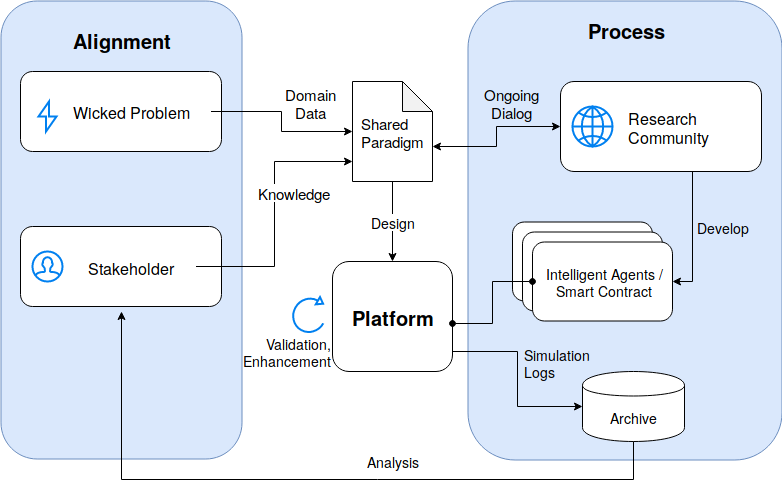
\includegraphics[width=1\linewidth]{./figures/competitive_benchmarking.png}
	\caption{Research Design following \protect\shortciteA{ketter2015competitive}}
	\label{figure:competitive_benchmarking}
\end{figure}

According to the IS Design Science principles introduced by Hevner, March, Park, and Ram \shortcite{hevner2008design}, 
the presented research design produce a viable artifact in the form of an open simulation platform, which depict a 
relevant real-world wicked problem. Due to the outcoming data produced by the simulation platform, 
it is possible to develop methods to evaluate the utility, quality and efficacy of the artifact. 
Moreover, the research provide a varifable contribution through the artifact, the open simulation platform, itself. 
The platform enables the investigation of possible solutions of unsolved problems and further, 
it removes the technical barriers for the use of the complex distributed ledger technology. 
Besides, the implementation of the platform is based on an appropriate selection of techniques. 
As stated in \ref{sec:Blockchain-based Energy Markets}, 
blockchains are a suitable technology to implement decentralized microgrid energy markets. 
In addition, the in \ref{sec:Distributed Resource Optimization} introduced distributed optimization 
algorithm achieve evidentially system optimality under a dynamic market-trading algorithm. 
Therefore, this research relies upon the application of rigorous methods and comply the requirement 
of the fifth guideline by \shortciteA{hevner2008design}. 
In addition, the platform enables the iterative search for an optimal design through the comparison 
of different produced solutions and is valuable to technology-oriented as well as management-oriented 
audiences. As a result, these research design also fulfil the seven research guidlines of 
the research framework introduced by \shortciteA{hevner2008design}. 


\section{Expected Contribution}
\label{sec:expected_contribution}

This research provides two different contributions. First, the fully decentralization of the introduced distributed optimization algorithm \shortcite{guo2007market}. 
The bundle-trading market grant access of any given trade to the market dealer. This, again, necessitates trust of the agents that it will use those resources according to the over-arching organizational goal. Due to the implementation of the market dealer by a smart contract, the technical implementation is public accesible. Moreover, all transactions of the market dealer to allocate the resources are transparent. Therefore, the behavior of the market dealer is comprehensible for every participant. Furthermore, it provides a high degree of security due to cryptographic encryption methods which are essential parts of the blockchain.
Second, the open simulation platform itself. From the scientific perspective, the platform is relevant due to the removal of existing technical barriers for practicioners in using complex distributed ledgers technologies. Therefore the platform facilitates researchers without a deep technically background to use those DLTs and incentivises to design and test their artifacts by using this platform. 
On the other hand, from a business perspective, this research is relevant to policy makers and energy suppliers. The platform allows stakeholders to get a better understanding of the dynamics of decentralized LEM and enables the testing and evaluating of policy options and implications. 

\clearpage

\section{Local Energy Markets}
\label{sec:lem}

\begin{figure}[htbp]
	\centering
	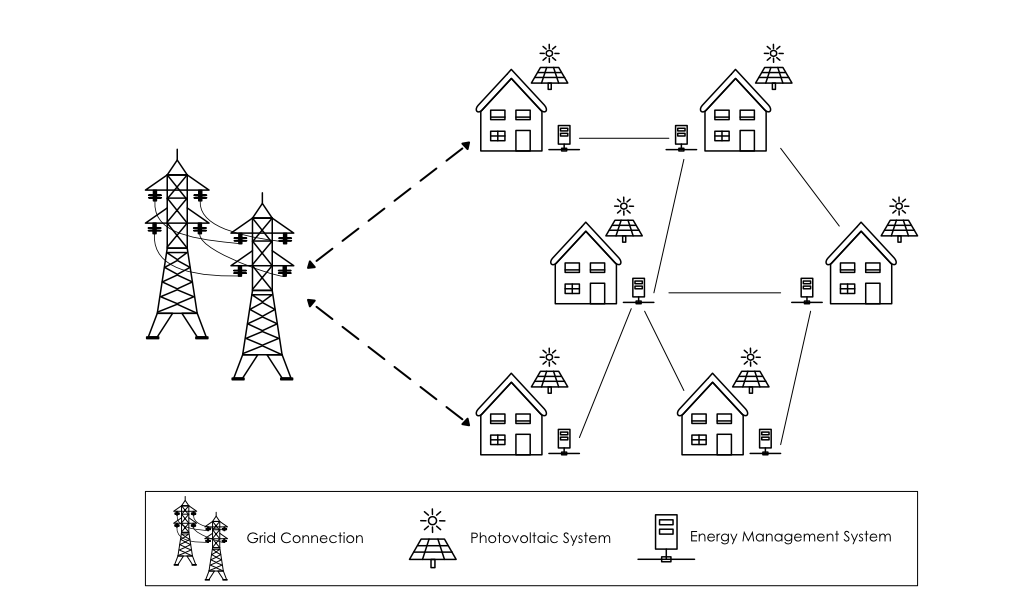
\includegraphics[width=.9\linewidth]{./figures/microgrid_1024x.png}
	\caption{Example of Microgrid setup taken from \protect\shortciteA{mengelkamp2018designing}}
	\label{figure:microgrid}
\end{figure}

To begin with, we revive the stated problem of successful integration of the increasing amount of
distributed RES, as already addressed 
in section \ref{sec:research_motivation}. Due to the centralized generation by large power plants
and the current design of the wholesale markets, the existing grid is not suitably designed
to react in real-time to a significant growing 
amount of distributed RES \shortcite{mengelkamp2018designing} \shortcite{ampatzis2014local}.

To successfully integrate and use these RES, new approaches are necessary \shortcite{mengelkamp2018blockchain}.
A possible solution to those technical and market problems is P2P energy 
trading in LEM \shortcite{long2017feasibility}. 

This section will explain the general concept of LEM
and present market components for building efficient LEM. 

In the traditional centralized energy system, large power plants that operate according to a
centralized coordination mechanism, supply a large amount of customer with energy, which are located 
within a wide area (for example a country or a state) \shortcite{mengelkamp2018designing}.

In contrast, decentralized energy systems consist of small-scale energy generators that are 
only used by a small number of people and located close to the energy consumption point \shortcite{mengelkamp2018designing}.
Those LEM provide a market platform, market mechanism, and market access
for small-scale prosumer and consumer, to trade locally generated energy within their community.
In this case, a community presents a group of geographically and socially close energy agents.
Moreover, all participants buy or sell energy directly with each other by using the provided market platform
without intermediation by conventional energy suppliers \shortcite{zhang2017review}.

In addition, if prosumer has a surplus in electricity, they have the opportunity 
to curtail it, store it in an energy storage device or export it back to the main power grid \shortcite{zhang2017review}.
Considering, in the traditional centralized energy system, trading of energy is mainly unidirectional.
As stated above, electricity is usually transmitted from large-scale power plants to 
consumers over long distances, while the cash-flow goes the opposite way. 
On the contrary, the P2P energy trading in a LEM encourages multidirectional trading within 
a local geographical community \shortcite{zhang2017review}, as illustrated in figure \ref{figure:microgrid}.

Due to this, LEM promote the consumption of energy close to its generation and, therefore, 
support sustainability and the efficient use of local resources \shortcite{mengelkamp2018designing}.
Furthermore, LEM enable (near) real-time pricing and facilitate a local balance
of supply and demand \shortcite{mengelkamp2018blockchain}. 

Further, as stated by \shortciteA{mengelkamp2018designing},
the participants of a LEM do not necessarily have to be physically connected. A virtual microgrid
describes the aggregated control of multiple energy producers, prosumers and consumers in a virtual 
community. Further, the revenue potential can be increased significantly by expanding a physical 
microgrid to include virtual participants. 

Referring to \shortciteA{jimeno2011architecture}, an LEM has a specific characteristic
that distinguishes it from other aggregation of DER systems. A microgrid has the opportunity
to operate either connected to the main grid or islanded from it. In other words,
this allows a LEM to run disconnected from the main grid, in case it fails or 
the power quality is not satisfactory. Thus, participants of a LEM have a higher quality 
of supply for the loads within it. Additionally, it offers a way of obtaining cheaper 
and cleaner energy for all participants, if elements operated in a LEM taking into 
account by economic and emission policies.

Moreover, P2P energy trading in a LEM requires advanced communication and data 
exchanges between the different parties, which makes central management and 
operation more and more challenging. The implementation of LEM needs 
local distributed control and management techniques. \shortcite{andoni2019blockchain}. 
\shortciteA{zhang2017review} stated that P2P energy trading is often
enabled by ICT-based online services. Moreover, \shortciteA{mengelkamp2018designing} explain that 
the new and innovative blockchain technology as an emerging ICT, 
offers new opportunities for decentralized market designs.
It is designed to enable distributed transactions without 
a central trusted entity.
Accordingly, blockchain can help to address the challenges faced by 
decentralized energy systems. 

\subsection{Components of local energy markets}
\label{sec:components_of_local_energy_markets}
\shortciteA{mengelkamp2018designing} developed in his research seven components for efficient
operation of blockchain-based LEM. This subsection will name and briefly 
illustrate each component. Further, the compliance of the developed open blockchain-based
LEM simulation and the seven components will be examined later on in section \ref{sec:compliance_of_components}.

\begin{description}
    \item[Microgrid setup (C1):] In general, an explicit objective, a definition of the market 
     participants and the form of the traded energy must be well defined. 
     A LEM can have different, often contradictory objectives. Especially in the
     design of the market mechanism, the implementation of the objective plays an important role.
     Next, a significant number of market participants is needed, who trade energy among each other.
     Moreover, a part of the market participants needs to be able to produce energy. 
     Finally, the form of the traded energy must be described, for example, electricity, heat or a 
     combination of them. Additionally, the way of energy transportation must be specified.
     Will be the traditional energy grid used or a physical microgrid build. 
    
    \item[Grid connection (C2:)] The connection points to the superordinate main grid 
     must be well defined. These points measure the energy flows towards the main grid 
     and evaluate the performance of the LEM and can help to balance the energy generation 
     and demand within it. Besides, you have to distinguish between a physical microgrid and 
     a virtual microgrid. A physical microgrid brings along a power distribution grid and is able to
     decouple from the main grid, whereas a virtual microgrid simply connects all participants over 
     an information system (C3). Consequently, a virtual microgrid does not have the opportunity
     to physically decouple from the main grid. 
     Nevertheless, to operate in island-mode extensively, a physical microgrid need a large 
     amount of own energy generation capacity and flexibility to ensure supply security and robustness.
         
    \item[Information system (C3):] In addition, all participants must be connected 
    and a market platform that monitors all operations must be provided. 
    Therefore, an information system is needed, which should enable equal 
    access for every market participant to avoid discrimination. 
    With reference to \shortciteA{mengelkamp2018designing}, these requirements
    can be implemented by blockchain technology based on smart contracts.
    
    \item[Market mechanism (C4):] Besides, a market mechanism implemented through 
     the information system is necessary. This market mechanism implies the allocation of the
     market and the payment rules. Further, a clear bidding format should be defined. 
     It follows that the main objective of the mechanism is to provide an efficient
     energy allocation by matching the buy and sell orders of the participants appropriately.
     Finally, this should happen in near real-time granularity.    
    
    \item[Pricing mechanism (C5):] The market mechanism (C4) includes the pricing mechanism 
     and supports the efficient allocation of energy supply and demand. 
     The traditional energy price is composed of large parts of taxes and surcharges.
     On the contrary, in a LEM different fees come to bear, for example in case of a 
     physical microgrid. Hence, RES typically have almost zero marginal cost, prosumer can 
     price their energy above all appropriate taxes and fees to make profit. 
    Thus, the energy price should be linked to the availability of energy. In other words,
    a surplus of energy should lower the LEM energy price while a lack of energy increases the 
    market price. From an economic point of view, LEM are beneficial to their 
    participants as long as the average energy price is lower than the external grid price.
        
    \item[Energy management trading system (C6):] The task and goal of the EMTS
     is to automatically ensure energy supply for a respective market participant.
     Therefore, the EMTS needs access to the energy-related data of the participant, like 
     the real-time demand and supply. The EMTS uses this data to forecasts consumption and
     generation and develops a bidding strategy accordingly. 
     Moreover, the EMTS trades the predicted amounts on the provided market platform 
     and aims to maximize the revenue and minimize the energy costs. 
     For this reason, the EMTS needs to have access to the market participant’s
     blockchain account to be capable to automatically perform energy transactions.

    \item[Regulation (C7):] It needs to be determined how a LEM 
     fit into the current energy policy and which market design is allowed, how 
     taxes and fees are distributed and billed. Likewise, it needs to 
     determined in which way the local market is integrated into the traditional
     energy market and energy supply system.
     All these emerging issues are specified by the legislative regulation.
    
\end{description}

\begin{comment}
    # Mengelkamp \shortcite{mengelkamp2018designing}
    
    An exemplary microgrid energy market scenario of residential consumers and 
    prosumers (consumers with photovoltaic (PV) systems) is shown in Fig. 2. 

\end{comment}

\clearpage

\section{About Blockchain}

To begin with, this chapter will give an overview of the general purpose, the contained components and the fundamental functionality of a blockchain. 

\subsection{General Purpose}
In general, a blockchain can be described as a digital data structure that can be understand as a shared and distributed database, containing a continuous expanding and chronological log of transactions \shortcite{andoni2019blockchain}. Besides, various types like digital transactions, data records and executables can be stored in this digital data structure. The data transmission in a blockchain is comparable with copying data from one computer to another. However, the resulting challenge is that the system needs to ensure that the data is copied just once \shortcite{andoni2019blockchain}. For example, in the domain of cryptocurrencies, this is equal to sending a coin from one wallet to another. In this case, the system needs to validate that this coin is spended just once and there is no double-spending. A conventional solution for this problem is a third intermediary. To come back to the stated example, the third intermediary is represented by a traditional bank, which store, protect and continuously update the valid state of the ledger \shortcite{andoni2019blockchain}. But, in some cases central management is not practicable or reasonable. Reasons for this are possible intermediary costs or a high degree of trust of the users into the intermediary who operates the system. Further, central management has a significant disadvantage because of a single point of failure. Hence, the centralized system is fragile to technical problems as well to external malicious attacks \shortcite{andoni2019blockchain}.
Consequently, the main reason of bockchain technologies is the removal of such third trusted intermediaries through a distributed network of various users, who cooperating together to verify transactions and protect the validity of the ledger

\subsection{Architecture}
This subsection covers the architectural design of a blockchain and presents the contained components in detail. Due to the plurality of the blockchain technologies, each of the technology slightly differs in design and components. The following explanations are oriented torwards the Ethereum blockchain implementation, which is also used as the underlying ICT to implement the open simulation platform.

\subsubsection{World State}
\label{sec:world_state}
Referring to the \textit{Yellow Paper} by \shortciteA{wood2014ethereum}, Ethereum can be seen as a transaction-based state machine. What does that mean? At the beginning, Ethereums state machine starting with a so called \textit{"genesis state"}. This is analogous to a blank sheet. On this state, no transactions have happened on the network. Next, transactions are executed and the state of the Ethereum world changes into a new state. Further, transactions are executed incrementally and morph it into some final state. Consequently, the final state is accepted as the canonical version of the world of Ethereum and represents at any times the current state.

\begin{figure}[htbp]
	\centering
	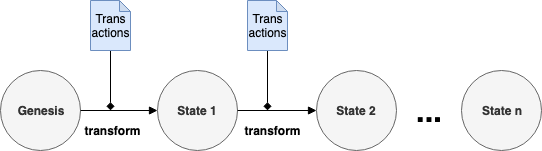
\includegraphics[width=.9\linewidth]{./figures/state_transition.png}
	\caption{World State: Transition of States}
	\label{figure:state_transition}
\end{figure}

In more detail, the world state arises out of a mapping of a key value pair for every account which exists on the Ethereum network \shortcite{wood2014ethereum}. The key constitutes the address of an Ethereum account and the value presents the account's state, which contains detailed information of this account. 
However, the world state is not stored on the blockchain itself. This mapping is stored and maintained in a modified data structure called a \textit{Merkle Patricia tree}. This tree is stored off-chain in a simple database backend (i.e. on a computer running an Ethereum client), also known as the \textit{state database} in the Ethereum world \shortcite{wood2014ethereum}. To get a better understanding of the operating principles of the blockchain, it is necessary to get an idea of how a \textit{Merkle Patricia tree} works. A \textit{Merkle Patricia tree} is a type of binary tree, which consists of a set of nodes. It has a large amount of 
\textit{leaf nodes}, containing the underlying data. Further, a set of intermediate nodes, where each node is the hash of its two children, and finally, one single root node, representing the top of the tree which is also build out of its two child nodes \shortcite{buterin2013next} \shortcite{wood2014ethereum}.
As mentioned before, the \textit{leaf nodes} contain the stored data by splitting these data into chunks. Afterwards, these chunks are splitted into buckets. Then, each bucket gets hashed and the same process repeats, traversing upwards the tree, until the total number of hashes remaining becomes only one and the root node is reached \shortcite{ethereum_blog}. 

\begin{figure}[htbp]
	\centering
	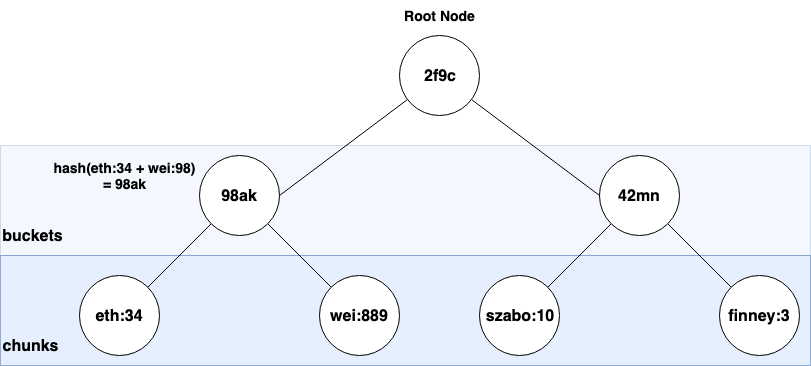
\includegraphics[width=.9\linewidth]{./figures/merkle_tree.png}
	\caption{Example of a Patricia Merkle tree}
	\label{figure:merkle_tree}
\end{figure}

Therefore, any change to the underlying data, stored in a \textit{leaf node}, causes a change of the hash of the node. Each parent's node hash depend on the data of its children. Due to this, any change to the data of a child node causes the parent hash to change. This procedure repeats traversing upwards until the root node. Hence, any change to the data at the leaf nodes effects the root hash \shortcite{ethereum_wiki}. 

\begin{figure}[htbp]
	\centering
	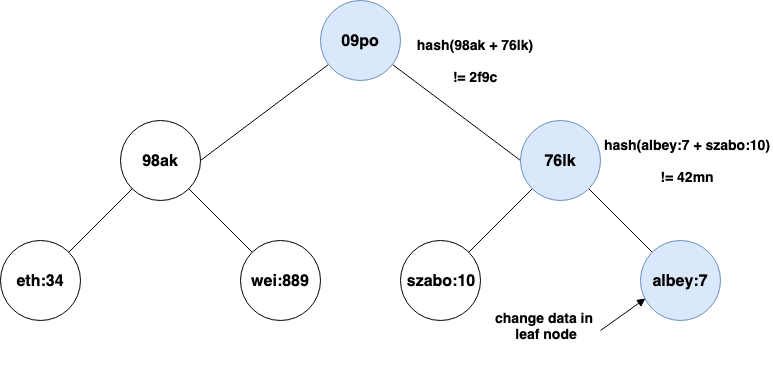
\includegraphics[width=.9\linewidth]{./figures/merkle_tree_change.png}
	\caption{Example of a data change in a leaf node}
	\label{figure:merkle_tree_change}
\end{figure}

Because of this characteristic, it is not necessary to compare the data of the entire tree. It is sufficient to compare the single root hash to ensure that all the data are the same. This property is very important, because it makes it possible to store only the hash of the root node to represent a state of the Ethereum world. 

\subsubsection{Block} 
\label{sec:block}
As described in section \ref{sec:world_state}, whenever transactions are executed, the state of the Ethereum world changes into a new state. Every state and the belonging transactions, which transform the prior state into the new state, is cumulated in a so called block. That means, states are represented by blocks. As you can see in figure \ref{figure:state_transition}, the history of the Ethereum world is a linkage of states, or in other words, blocks. That is where the name blockchain comes from. A blockchain is a sequence of blocks, which holds a complete list of transaction records \shortcite{zheng2017overview}. 
Moreover, a block is a collection of different relevant informations and consists of the \textit{block header} and the \textit{block body}, which contains the list of transactions. Following \textit{Ethereums Yellow Paper} by \shortciteA{wood2014ethereum}, the subsequent pieces of information are contained in the \textit{block header}:

\begin{description}
	\item[Parent Hash:] This is the hash of the parents block's header. Therefore, every block points to his ancestor. Due to this contained attribute, a chain arises out of the single blocks.
	\item[Beneficiary:] The miners address to which all block rewards from the successful mining of a block are transferred.
	\item[State Root:] This is the hash of the root node of the state tree, after a block and its transactions are finalized. As mentioned in section 
	\ref{sec:world_state}, the state tree is the one and only global state in the Ethereum world. It is used as a secure unqiue identifier for the state and the state root node is cryptographically dependent on all internal state tree data.
	\item[Transactions Root:] This is the hash of the root node of the transaction tree. This tree contains all transactions in the block body. In contrast to the state tree, there is a separate transactions tree for every block. 
	\item[Receipts Root:] Every time a transaction is executed, Ethereum generates a transaction receipt that contains information about the transaction execution. This field is the hash of the root node of the transactions receipt tree and like the transaction tree, there is a seperate receipt tree for every block.
	\item[Difficulty:] This is a measure of how hard it was to mine this block – a quantity calculated from the previous block’s difficulty and its timestamp
	\item[Number:] This is a quantity equal to the number of blocks that precede the current block in the blockchain.
	\item[Gas Limit:] This is a quantity equal to the current maximum gas expenditure per block. Each transaction consumes gas. The gas limit specifies the maximum gas that can be used by the transactions included in the block. It is a way to limit the number of transactions in a block.
	\item[Gas Used:] This is a quantity equal to the total gas used in transactions in this block.
	\item[Timestamp:] This is a record of Unix’s time at this block’s inception.
	\item[Nonce:] This is an 8-byte hash that verifies a sufficient amount of computation has been done on this block. Further, it is a number added to a hashed block that, when rehashed, meets the difficulty level restrictions. The nonce is the number that blockchain miners are solving for.
\end{description}

So far, we introduced Ethereum as a transaction-based state machine, transforming one state into another through the execution of transactions. Further, we explained how these individual states are stored and emphasises the meaning of these storage. Moreover, we pointed out that an Ethereum state is represented by blocks and described all relevant informations contained in it.
However, we didn't introduce how many transactions be part of a block and who build and validate a block? To answer this, we introduce the transaction object and his life cycle in depth.


\subsubsection{Transaction}
\label{sec:transaction}
To start with, a transaction is the basic method for Ethereum accounts to interact with each other. Further, in the Ethereum world exists two different types of transactions. Those, which result in a so called \textit{message call}, which can be seen as a traditional transaction, and those which result in a \textit{contract creation} \shortcite{wood2014ethereum}. 
Though, both different types of transaction share the following common attributes \shortcite{wood2014ethereum}:

\begin{description}
	\item[Nonce: ] This attribute is discontiguous of the block attribute. In contrast to the block attribute, the nonce of a transaction keep track of the total number of transactions that an account has executed. 
	\item[Gas Price: ] As mentioned in section \ref{sec:block}, each transaction consume gas. Gas can be seen as fees. This attribute presents the price per unit of gas for a transaction \footnote{A website to see current gas prices: https://ethgasstation.info/index.php}. 
	\item[Gas Limit: ] This attribute is similiar to the block attribute of the same name. In this case, it is a quantity equal to the current maximum gas expenditure per transaction.  
	\item[To: ] In case of a \textit{message call}, this attribute contains the address of the recipient. Otherwise, in case of a \textit{contract creation} this value remains empty. 
	\item[Value: ] In case of a \textit{message call}, this attribute contains the amount of Wei, which will be transferred to the recipient. In the case of a \textit{contract creation}, this value contains the amount of Wei as a intial endowment of the contract.
\end{description}

\subsubsection{Transaction Life Cycle}
\label{sec:transaction_lifecycle}
Next, the life cycle of a transaction will be outlined. We will take a simple \textit{message call} as an example and will pass through the entire flow of how this transaction gets executed and permanently stored on the blockchain. During this process, many basic concepts of a blockchain will be introduced. 

To begin with, someone want to send an abitrary amount of ether to someone else. 
Consequently, a transaction with the respective attributes, which are stated 
in section \ref{sec:transaction}, will be created. As a first step, this transaction 
will be signed. That means, the one who wants to execute the transaction needs to proof the 
ownership of the account. Otherwise, someone else could execute a transaction on your behalf. 
The way to proof this is by signing the transaction with the corresponding private
key of this account \shortcite{transaction_life_cycle}. 
Next, the signed transaction is submitted to the related Ethereum node. 
Then, the node will validate the signed transaction. 
After a successful validation, the node will send the transaction to 
it's peer nodes, who again send it to their 
peer nodes and so on \shortcite{transaction_life_cycle}. 
As soon as the transaction is broadcast to the network, 
the related node will declare a transaction id, which is the hash 
of the signed transaction and can be used to track the 
status of the transaction \footnote{A Website to track transactions: https://etherscan.io/}. 

\begin{figure}[htbp]
	\centering
	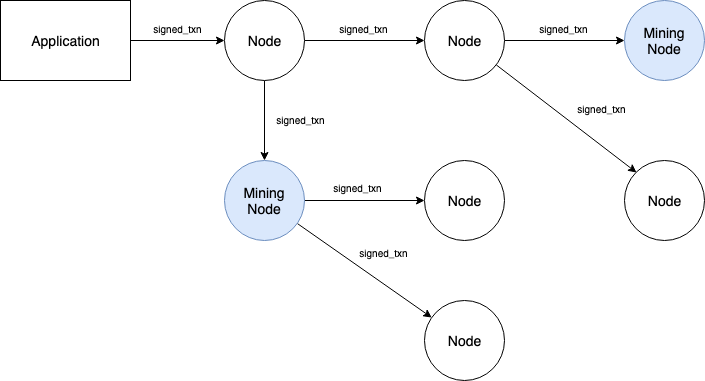
\includegraphics[width=.9\linewidth]{./figures/node_network.png}
	\caption{Node network demonstrating a transaction broadcast}
	\label{figure:node_network}
\end{figure}

\clearpage

Further, figure \ref{figure:node_network} describes a Ethereum network. 
As you can see, it contains a mix of miner nodes and non miner nodes. 
The non miner nodes can be distinguished into different types of nodes with different 
behavior, which are explained in detail in section \ref{sec:nodes}. 
The miner nodes are the ones who processing transactions into blocks \shortcite{transaction_life_cycle}. 

Mining nodes contain and maintain a pool of transactions where they collect incoming transactions. 
They sort the transactions by gas price. 
However, there are no specific rules how the nodes sort the transactions. 
A common configuration is to sort the transaction by gas price in a descending order to 
optimize for a higher pay \shortcite{transaction_life_cycle}.

\begin{longtable}{c|c}
	\hline
	Signed Transaction & Gas Price \\
	\hline
	hashOfTransaction1 & 15 Gwei \\
	hashOfTransaction2 & 13 Gwei \\
	hashOfTransaction3 & 11 Gwei \\
	hashOfTransaction4 & 10 Gwei \\
	hashOfTransaction5 & 7 Gwei \\
	\hline
	\caption{Transaction Pool of Mining Node}
	\label{table:sorted_gas_prices}
\end{longtable} 

Further, the mining node takes transactions from the pool and processes them into a pending block. 
Moreover, a block can only contain a certain number of transactions due to the block 
attribute \textit{gas limit}, mentioned in section \ref{sec:block}. 
That means, the mining node can only process so many transactions into one 
block until the gas limit is reached \footnote{A website to see 
current attributes: https://ethstats.net/}. For example, 
imagine that the current \textit{gas limit} of a block is 28 Gwei. 
Next, we look at the transaction pool of a mining node in 
table \ref{table:sorted_gas_prices}. As you can see, two blocks are 
required to process all transactions from the pool. The first two transactions 
are contained in the first block. Furhtermore, the second block contains the remaining 
three transactions. 
So far, it is described how a pending block will be created and the transaction 
limit of a block is explained. In the next section \ref{sec:mining}, 
the process of a pending block to a valid block is outlined in depth. 
Finally, after the validation process of a block is finished successfully, 
the life cycle of a transaction is terminated. In other words, the transaction is anchored 
in the blockchain and modified the world state as mentioned in section \ref{sec:world_state}.

\subsubsection{Mining}
\label{sec:mining}
In this section, the stteps of the validation process of a pending block will be described. 
In general, each mining node in the network can generate or propose a block. 
The emerging question is, which node build the new block and how will the newly 
generated block accepted by the remaining network members? 
This process is called \textit{consensus mechanism}.
It exists a lot of various consensus algorithms, each of them provides different features,
advantages and disadvantages. 

To a large extent, the key perfomance drivers of a blockchain
like transaction speed, scalability and security depending on the embedded consensus algorithm \shortcite{andoni2019blockchain}. 
In this section, we will expound the \textit{Proof of Work (PoW)} mechanism, 
which is at the time of this writing the current strategy in the Ethereum blockchain 
implementation for reaching consensus. 
\textit{Proof of Work} enables a high scalability in terms of the number 
of nodes and clients \shortcite{vukolic2015quest}, whereas it provides a poor transaction speed and a high 
power consumption due to the solving of a cryptographical puzzle, which requires 
significant computational effort \shortcite{andoni2019blockchain}. 

% erklärung crypthograpgical puzzle
The \textit{PoW} is a random process which is not predictable and therefore only solvable through a 
trial and error approach \shortcite{bitcoin_wiki_pow}. 
All mining nodes compete with each other and the goal is to achieve a hash output that 
is lower than a given specified target \shortcite{andoni2019blockchain}.
The hash output includes and comprises out of the \textit{Parent Hash}, \textit{Transaction Root} and
\textit{Nonce}, which are all part of the block headers data, mentioned in \ref{sec:block}.
However, the \textit{Parent Hash} and \textit{Transaction Root} are given and immutable, thus the \textit{Nonce}
is the value that all the mining nodes are solving for \footnote{A interactive blockchain demo: https://anders.com/blockchain/}.
Consequently, the mining nodes modify the \textit{Nonce} until the hash output is lower than the required target \shortcite{andoni2019blockchain}.
The following pseudocode in listing \ref{lst:pow_mechanism} will illustrate the \textit{PoW} procedure:

\vspace{7mm}
\begin{lstlisting}[label={lst:pow_mechanism}, caption={Pseudocode for PoW mechanism}]
	targetValue = 00005cdf6d384113165841052dfd4638eaf756ac
	parentHash = abbecf2d59eacbde676c3f1f0bfcf124f8c68209
	transactionRoot = 917c631e5ee59596859910759c8ed76a21252010
	nonce = 1
	valid = False

	while(not valid):
			hashOutput = sha256(parentHash+transactionRoot+nonce)
		
			if(hashOutput <= targetValue):
					valid = True
			else:
					nonce += 1

\end{lstlisting}
\clearpage

Finally, when one mining node successfully calculated the \textit{Nonce} and therefore reaches the target value, 
it broadcasts the block to all other mining nodes in the network. Now, all other nodes mutually validate the correctness of the hash value
by recalculating the hash output and verifying if it is lower then the target value. 
If the block is validated through all other mining nodes, all nodes will append this new block to their own blockchains \shortcite{zheng2017overview}.  

% erklärung multiple chains
Considering, the network is decentralised and the simultaneous generation of valid blocks is possible when multiple nodes find 
the suitable \textit{Nonce} at a nearly same time \shortcite{zheng2016blockchain}. In this case, branches will be generated as shown in figure \ref{figure:blockchain_branches}

\begin{figure}[htbp]
	\centering
	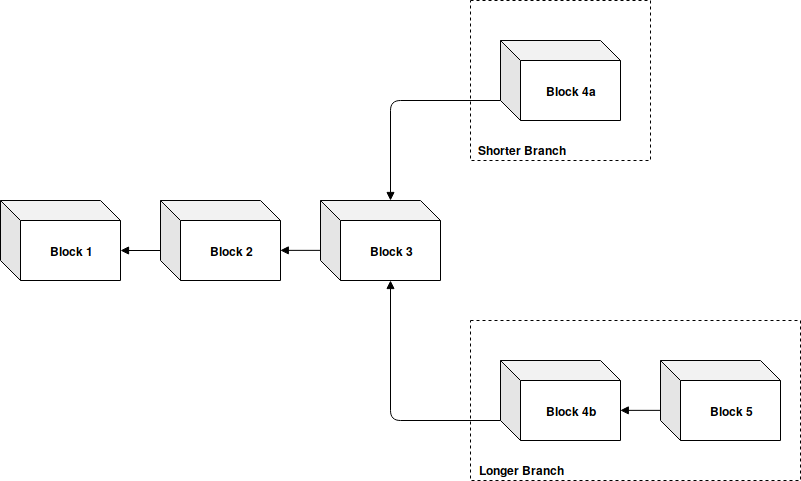
\includegraphics[width=.9\linewidth]{./figures/blockchain_branches.png}
	\caption{Scenario of Blockchain Branches}
	\label{figure:blockchain_branches}
\end{figure}

Nevertheless, it is unlikely that two competing branches will generate the next block simultaneously again. 
In the \textit{PoW} protocol, the longer branch is judged as the authentic one. 
In figure \ref{figure:blockchain_branches}, two branches arised out of 
two simultaneous valided blocks \textit{Block 4a} and \textit{Block 4b}. 
After that, all mining nodes accept both branches and start working on 
the next consecutive block until a longer branch is found \shortcite{andoni2019blockchain}. 
As you can see in figure \ref{figure:blockchain_branches}, \textit{Block 4b} and \textit{Block 5} forms the longer 
chain, therefore all miners on the branch with \textit{Block 4a} will switch to 
the longer branch \shortcite{zheng2017overview}. 

To sum up, this section joins and completes the previous section \ref{sec:transaction_lifecycle}.
The consensus mechanism \textit{PoW} is described and outlined in pseudocode, whereby
the validation process of new generated blocks is explained and illustrated.
\clearpage

\subsubsection{Ethereum Clients}
\label{sec:nodes}

First of all, the expressions Ethereum client and Ethereum node can be used interchangeable. 
As mentioned earlier in the previous section \ref{sec:transaction_lifecycle} 
and illustrated in the figure \ref{figure:node_network}, clients can be distinguished into different types. 
This section will describe the concept of an Ethereum client in general and will give a brief overview of the different
types.

In general, an Ethereum client is a software application 
that implements the Ethereum specification, which is specified in the Ethereum yellow paper \shortcite{wood2014ethereum}.
A client communicates over the peer-to-peer network with other Ethereum clients.
Although these clients can be implemented in different programming languages, they all communicate through
the standardized Ethereum protocol, wherefore they are able 
to operate and interact with the same Ethereum network. \shortcite{antonopoulos2018mastering}. 

Since the Ethereum blockchain is not officially implemented in a particular programming language, 
following a list of the current main implementations of the Ethereum protocol:

\begin{itemize}
	\item \texttt{Parity}, written in Rust
	\item \texttt{Geth}, written in Go
	\item \texttt{cpp-Ethereum}, written in C++
	\item \texttt{pyethereum}, written in Python
	\item \texttt{Harmony}, written in Java 
\end{itemize}

However, while all clients differ from each other, they share some fundamental features \shortcite{ethereum_clients}.

First, each is able to join the peer-to-peer Ethereum network. 
Next, they all synchronizing a local copy of the blockchain.
There are a few modes of synchronizing, which comes with miscellaneous advantages and disadvantages, 
which will be outlined later on. Moreover, it makes a significant difference 
for the health and resilience of the decentralised network. 
Lastly, each client is also capable of broadcasting new transactions to the network and creating and 
managing accounts \shortcite{ethereum_clients}.

As mentioned above, there are differences in client behavior regarding to the synchronizing modes. 
In general, the clients can be distinguished into two different types, the so called \textit{full node} and 
\textit{light node}. 

\paragraph{Full Node:} A full node will download all history data peer-to-peer from
another full node. This requires a significant amount of hardware and bandwith resources \shortcite{antonopoulos2018mastering}.
Afterwards, it will simulate every transaction in the ledger
and execute the whole deployed source code to recalculate the state of each existing block \shortcite{ethereum_clients}.
Therefore, the amount of independently operating and geographically dispersed full nodes 
is a crucial and very important indicator for the health, resilience and 
censorship resistance of a blockchain \shortcite{antonopoulos2018mastering}. 
However, a full node is not necessarily a mining node. It authoritatively validates all transactions, but 
to participate in the mining competition, an additional software called \textit{ethminer}
 is needed \footnote{GPU Mining Worker: https://github.com/ethereum-mining/ethminer}

\paragraph{Light Node:} To begin with, a light node is not a separate piece of software from the clients that 
run a full node. The difference lies in the \textit{light} mode for synchronization. 
In contrast to a full node, a light node only synchronize the block headers and the 
current state of the chain \shortcite{ethereum_light_node}.
Anyway, a light node lacks the ability to run transactions throughout the history of the 
whole blockchain. For this reason, it does not contribute to the health and resilience of 
the network like a full node and traditionally cannot act as a mining node \shortcite{ethereum_clients}. 
In addition, a light node has some further limitations. For instance, they are not 
capable to monitor pending transactions from the network and the hash of a transaction
is not sufficient to locate the transaction. Moreover, to perform certrain types of operations,
a light node relies on requests to full nodes, whereby they can be far slower to query the chain \shortcite{ethereum_light_node}.


\subsubsection{Smart Contract}

This section deals with smart contracts in the Ethereum world and based 
entirely on the book \textit{Mastering Ethereum} by \shortciteA{antonopoulos2018mastering}.
First of all, the term smart contract is a bit misleading, since Ethereum smarts contract 
are neither smart nor legal contracts. However, how can a Ethereum smart contract be defined?
A Ethereum smart contract is an immutable comuputer program that runs deterministically in the context of an
Ethereum Virtual Machine (EVM) as part of the networkprotocol. To go into the definition in more detail, 
immutable means, that once the contract is deployed into the blockchain, it is not possible to make any
changes in the source code. The only way to modify the contract is to deploy a whole new instance. 
Further, deterministic means that the result of the execution is the same for all who run it, 
depending on the context of the transaction that initiated its execution and the state of the blockchain
at the moment of execution.
As already mentioned in section \ref{sec:transaction}, in the Ethereum world exists two different types of transactions.
Those which result in a message call, and those which result in a contract creation. 
That means, smart contracts are deployed through special contract creation transactions into the blockchain. 
The special thing about these transactions is that the recipient of the transaction remains empty, whereby the transaction
will be send to a special destination address called \textit{zero address (0x0)}. Each contract is identified and reachable via
a common Ethereum address, which can be used in a transaction as the recipient to send funds to the contract or to call 
one of the contract functions. Anyway, in contrast to an externally owned account, there are no keys associated with 
an account of a smart contract. For this reason, the creator of a smart contract does not have any special rights at the 
protocol level. Although, it is possible to get those special rights if you explicitly 
specified them in the source code of the contract.
Furhtermore, contracts are only active and run if they called by a transaction. 
A contract is able to call another contract and so on, but nevertheless, 
the first call have always come from an externally owned account. 
A contract will never run on his own or in the background. Additionally, contracts are not executed in parallel.
They will always executed consecutively, hence the Ethereum blockchain can be considered as a single-threaded machine. 
Finally, it should be noted that transactions are atomic regardless of how many contracts they call. Transactions execute in
their entirety and any changes in the global state are only recorded if all executions terminates successfully. 
If the executions fails, all the changes in state are reverted as if the transaction never ran. Anyhow, a failed
execution of a transaction is recorded as having been attempted. Moreover, the gas fees spent for the execution is withdrawn
from the originating account.

\clearpage

\section{Linear Programming}
\label{sec:linear_progamming}
This section will give an introduction into the basics of mathematical linear programming
and linear programming duality.
It will present the purpose and necessity of optimization models and will give
an example of how an optimization model is constructed. 

To begin with, optimization models try to define in mathematical terms, the goal
of solving a problem in the best or optimal way. 
This can be applied in many different areas, for example, it might mean running a business to 
maximize profit, designing a bridge to minimize weight or selecting a flight plan for an aircraft
to minimize time or fuel use \shortcite{griva2009linear}. 
The use case of solving an optimization problem optimally is so ubiquitous, 
that optimization models are used in almost every area of application \shortcite{griva2009linear}.
Often it is not possible or economically feasible to make decisions without the help
of such a model. Due to the excellent improvements in computer hardware and software
in the last decades, optimization models became a practical tool 
in business, science and engineering \shortcite{griva2009linear}. 
Finally, it is possible to solve optimization problems with a huge set of variables. 

Further, linear optimization, also known as a \textit{linear program (LP)}, refers to the optimization
of a linear function with the decision variables, $x_{1}, ..., x_{n}$ subject to 
linear equality or inequality constraints. 
As presented by \shortciteA{bichler2017market}, in canonical form 
a linear optimization model is given as:

\begin{equation*}
    \begin{array}{ll@{}ll}
        \text{max}  & \displaystyle\sum\limits_{j=1}^{n} c_{j}x_{j} &\\
        \text{s.t.}& \displaystyle\sum\limits_{j=1}^{n} a_{ij}x_{j} \leq b_{i},  &&i=1 ,..., m\\
                    &                        x_{j} \geq 0, &&j=1 ,..., n
    \end{array}
\end{equation*}

However, a LP can be modeled in different forms. It is also possible 
to write a model in the matrix-vector notation. To represent the above model in this form, letting
$x=(x_{1}, ..., x_{n})^{T}$, $c=(c_{1}, ..., c_{n})^{T}$, $b=(b_{1}, ..., b_{m})^{T}$
and name the matrix of the coefficients $a_{ij}$ by $A$. As introduced by \shortciteA{griva2009linear},
the model becomes:

\begin{equation*}
    \begin{array}{ll@{}ll}
        \text{max}  & \displaystyle c^{T}x &\\
        \text{s.t.}& \displaystyle Ax \leq b&\\
                    &                        x \geq 0
    \end{array}
\end{equation*}

\clearpage
In general, the objective function of a linear model is either minimized or maximized.
Additionally, the constraints may include a combination of inequalities and equalities
and the variables are unrestricted or restricted in sign \shortcite{bichler2017market}.

\subsection{Duality Theory}
\label{sec:duality_theory}
In addition, for every LP exists another problem, which
is called the \textit{dual} of the original linear problem, also known as the 
\textit{primal} \shortcite{bichler2017market}.
In the dual, the roles of variables and constraints are reversed. 
That means, every variable of the primal becomes a constraint in the dual,
and every constraint in the primal becomes a variable in 
the dual \shortcite{griva2009linear}.
For instance, if the primal has $n$ variables and $m$ constraints, the dual
will have $m$ variables and $n$ constraints. Further, the primal objective coefficients 
are the coefficients on the right-hand side of 
the dual, and vice versa.
Finally, the transposed coefficient matrix of the primal constitutes the matrix in the 
dual \shortcite{griva2009linear}.
To give an example of a primal and the corresponding dual LP,
the representation by \shortciteA{bichler2017market} is considered:

\begin{equation}
    \tag{primal}
    \begin{array}{ll@{}ll}
        \text{min}  & \displaystyle c^{T}x &\\
        \text{s.t.}& \displaystyle Ax \geq b  &\\
                    &                        x \geq 0
    \end{array}
\end{equation}

\begin{equation}
    \tag{dual}
    \begin{array}{ll@{}ll}
        \text{max}  & \displaystyle b^{T}y &\\
        \text{s.t.}& \displaystyle A^{T}y \leq c &\\
                    &                        y \geq 0
    \end{array}
\end{equation}


Next, the motivation of the duality theory can be explained by the issue of trying to find 
bounds on the value of the optimal solution to a LP. 
If the primal is a minimization problem, the dual represents a lower bound
on the value of the optimal solution, otherwise, if the primal is a maximization problem,
the dual represents an upper bound \shortcite{bichler2017market}.
To illustrate the concept and motivation of duality theory more tangibly, an example stated by 
\shortciteA{bichler2017market} is given. 
In an application, the variables in the primal linear problem stand for consumer products and
the objective coefficients represent the profits linked to the production of those consumer products. 
In this case, the objective in the primal describes directly the relation between a change
in the production of the products and profit. Whereas, the constraints in the primal 
describe the availability of raw materials. Consequently, an increase in the availability of 
raw materials needed for the production of the consumer products enables an increase in production,
and finally an increase in the overall profit. 
However, the primal problem does not outline this relationship reasonable. Hence, one of 
the benefits of the dual is to properly show the effect of changes in the constraints on the
value of the objective. Due to this, the variables in a dual LP often called 
\textit{shadow prices}, since they describe the hidden costs associated with the constraints. 

\subsubsection{Weak Duality Theorem}
As stated in the section before (\ref{sec:duality_theory}), the \textit{dual} problem 
provides, depending on maximization or minimization problem, lower and upper bounds for 
the \textit{primal} objective function. Referring to \shortciteA{vanderbei2015linear},
this result is true in general and is described as the \textit{Weak Duality Theorem}:

\begin{theorem}
    If $x$ is feasible for the primal and 
    $y$ is feasible for the dual, then:

    \begin{equation*}
        \begin{array}{ll@{}ll}
            \displaystyle c^{T}x \leq b^{T}y&\\
        \end{array}
    \end{equation*}    

\end{theorem}

Regarding to \shortciteA{griva2009linear}, there are some logical corollaries 
of the Weak Duality Theorem:

\begin{corollary}
    If the primal is unbounded, then the dual is infeasible. 
    If the dual is unbounded, then the primal is infeasible.
\end{corollary}

\begin{corollary}
\label{strong_duality_corollary}
    If $x$ is a feasible solution to the primal, 
    $y$ is a feasible solution to the dual,
    and $c^{T}x = b^{T}y$, then x and y are optimal for their respective problems.
\end{corollary}

\subsubsection{Strong Duality Theorem}
\label{sec:strong_duality_theorem}
Concerning corollary \ref{strong_duality_corollary}, it is possible to verify if 
the points x and y are optimal solutions, without solving the corresponding LPs. 
Furthermore, this corollary is also used in the proof of strong duality \shortcite{griva2009linear}. 
The \textit{Strong Duality Theorem} describes, that for linear programming there 
is never a gap between the primal and the dual 
optimal objective values \shortcite{vanderbei2015linear}.

\begin{theorem}
    If  the primal problem has an optimal solution $x^{*}$,
    then the dual also has an optimal solution $y^{*}$,
    such that:

    \begin{equation*}
        \begin{array}{ll@{}ll}
            \displaystyle c^{T}x^{*} = b^{T}y^{*}&\\
        \end{array}
    \end{equation*}    

\end{theorem}

\subsubsection{Simplex-Method}
This subsection will give a brief introduction to the \textit{simplex-method}. 
To start with, in the field of linear programming, the simplex-method 
is the most widely used algorithm. 
This method was developed around 1940 and had several competitors at that time.
However, the algorithm was able to assert itself due to its efficiency. \shortcite{griva2009linear}
In general, the simplex-method is an iterative algorithm, used to solve 
a LP \shortcite{griva2009linear}. To apply the algorithm to a LP, 
it must be in standard form \shortcite{Luenberger2008}. According to \shortciteA{griva2009linear}, 
we consider the following LP:

\begin{equation*}
    \begin{array}{ll@{}ll}
        \text{min}  & \displaystyle z = -x_{1} - 2x_{2} &\\
        \text{s.t.}& \displaystyle - 2x_{1} + x_{2} \leq 2 &\\
                    & \displaystyle - x_{1} + 2x_{2} \leq 7 &\\
                    & \displaystyle  x_{1} \leq 3 &\\
                    &                        x_{1}, x_{2} \geq 0
    \end{array}
\end{equation*}

Next, we give an example to illustrate how to convert a LP into standard form.
To achieve that, the so-called \textit{slack variables} will be added, which represents the 
difference between the right-hand side and the left-hand side. 

\begin{equation*}
    \begin{array}{ll@{}ll}
        \text{min}  & \displaystyle z = -x_{1} - 2x_{2} &\\
        \text{s.t.}& \displaystyle - 2x_{1} + x_{2} + x_{3} = 2 &\\
                    & \displaystyle - x_{1} + 2x_{2} + x_{4} = 7 &\\
                    & \displaystyle  x_{1} + x_{5} = 3 &\\
                    &                        x_{1}, x_{2}, + x_{3}, + x_{4}, + x_{5} \geq 0
    \end{array}
\end{equation*}


Finally, with the LP in standard form, the idea of the simplex-method
is to iteratively proceed from one basic feasible solution to another \shortcite{Luenberger2008}.
Thereby, it always looks for a feasible solution which is better than the one before. 
The definition of better, in this case, depends on the nature of the linear problem. 
The process is performed until a solution is reached, which cannot 
be improved anymore. In the end, this final solution is then an optimal solution \shortcite{vanderbei2015linear}. 


\clearpage






\section{The Bundle-Trading-Market Framework}
\label{sec:btm}
To start with, we explained in section \ref{sec:lem} that local energy markets enable the trading 
of locally generated energy through a market platform, market mechanism and market access for 
small-scale prosumer and consumer. 
In addition, we presented in section \ref{sec:components_of_local_energy_markets} 
a market mechanism as one of seven core components for a efficient operation of blockchain-based
local energy markets.

On account of that, this chapter covers and explain in detail the applied market mechanism in the 
developed open blockchain-based LEM platform. 

As already briefly introduced in the sections \ref{sec:research_motivation} 
and \ref{sec:Distributed Resource Optimization}, the applied market mechanism is implemented 
through the developed market-based optimization algorithm, which is also called the 
\textit{bundle trading market framework} or short \textit{BTM}. 
In the proposed framework by \shortciteA{guo2012computational}, independent, self-interested
agents trading bundled resources in a double-auction market, which run by a dealer. 
In this case, the dealer replaces the central authority and agents represent distributed
entities. Generally, the \textit{BTM} consists of a master problem that solves 
the market-matching problem, which is managed by the dealer, 
and  subproblems that solve the bundle-determination problem of the agents.
Further, the solution process is an iteration between the market-matching problem and the 
the bundle-determination problems \shortcite{guo2007market}.
Considering, the \textit{BTM} constitutes a market-based decomposition method 
for decomposable linear systems,
which can be easily implemented to support real-time optimization 
of distributed systems \shortcite{guo2007market}.
Likewise, the central problem of the stated market-based optimization algorithm can 
interpreted as the welfare optimization of all participants in a LEM. 
The dealer, which runs the double auction market, maximizes the welfare through allowing 
agents to trade their preferable bundles of energy.
Therefore, the \textit{BTM} is a suitable market mechanism 
for the concept of a LEM and will be used as such in the developed blockchain-based LEM 
simulation platform. 

\subsection{Problem Overview}
\label{sec:btm_problem_overview}
This subsection will give an introductory description to the overall problem. 
With reference to \shortciteA{guo2012computational}, we consider a distributed 
system with $k$ independent agents.
In addition, we have a central problem and individual 
problems of the $k$ individual agents, which both can be expressed as the following 
linear programs. Besides, the \textit{BTM} presented by \shortciteA{guo2007market} requires 
a nondegenerate central problem with a bounded solution. In contrast to discrete markets where 
only integer number of units can be traded, the proposed framework facilitate continuous 
trade amounts. 

\paragraph*{Central Problem}
\begin{equation}
    \begin{array}{ll@{}ll}
        Z(c) = \underset{x_{j} \geq 0}{\text{min}}  & \displaystyle\sum\limits_{j=1}^{k} d^{T}_{j}x_{j} &\\
        \text{s.t.}& \displaystyle N_{j}x_{j} \leq n_{j}, &&i=1 ,..., k  \\
                    & \displaystyle\sum\limits_{j=1}^{k} C_{j}x_{j} \leq c
    \end{array}
\end{equation}

\paragraph*{Agent Problem ($j=1, ..., k$)}
\begin{equation}
    \begin{array}{ll@{}ll}
        z_{j}(c_{j}) =  \underset{x_{j} \geq 0}{\text{min}}  & \displaystyle d^{T}_{j}x_{j} &\\
        \text{s.t.}& \displaystyle N_{j}x_{j} \leq n_{j}, &&\\
                    & \displaystyle\sum\limits_{j=1}^{k} C_{j}x_{j} \leq c_{j}
    \end{array}
\end{equation}

In the table below, the applied variables in the stated equations are described:


\begin{longtable}{c|l}
	\hline
    $d_{j} \in R^{b_{j}}$ & vector of agents $j's$ costs \\
    $x_{j} \in R^{b_{j}}$ & decision variables controlled by agent j \\
    $N_{j} \in R^{a_{j} \times b_{j}}$ & activity matrix \\
    $C_{j} \in R^{m \times b_{j}}$ & activity matrix \\
    $n_{j} \in R^{a_{j}}$ & capacity vector of agent $j's$ independent resources that are managed locally \\
    $c_{j} \in R^{m}$ & agent $j's$ vector of shared resources that can be exchanged with other agents \\
	\hline
	\caption{Applied variables in BTM Framework}
	\label{table:applied_variables_in_btm}
\end{longtable} 

Further, the overall objective of the central problem is to minimize the 
operating costs of the overall system. The minimization of the central problem
have to be implemented in consideration of the operational constraints 
(first set of constraints) and the total shared 
resources capacity constraints (second set of constraints) of each individual agent. 
Anyhow, the optimal solution to the central problem cannot be directly calculated, 
due to the lack of access to all relevant information for decision making
($d_{j}, n_{j}, c_{j}, N_{j}, C_{j}, for j=1, ..., k$). 
Additionally, \shortciteA{guo2007market} stated that, for an allocation of 
$c_{j}, j=1, ..., k$ such that $C_{j}x_{j}^{*} \leq c_{j}, \sum\limits_{j=1}^{k} C_{j}$, 
solving the agents’ problems is equivalent to solving the central problem.

Hence, a market-based resource allocation mechanism to coordinate decentralized
decision making from agents is used by the \textit{BTM}. 
For any intially given $c_{j}, j=1, ..., k$, these mechanism enables an indirectly 
acquisition of an optimal solution to the central problem through an direct, iterative and
wealth-improving bidding process among the self-interested agents. 


\subsection{Market Environment}
Generally, a dealer and $k$ independent agents constitute the whole market economy. 
Each of the agent have the opportunity to trade the shared resources $c_{j}$ 
in a double auction market, which is operated by the dealer. Moreover, each agent 
only has local perspective and knowledge, that is to say, they don't know anything about 
the prodcution decisions of the others. 
Further, the market prices to match the trades, will be determined by the dealer.
Subsequently, the roles of the market participants and what they know is described. 
Equally, the market operations like the agent bidding, market matching and settlement 
is outlined and a summary of the market-based algorithm is presented. 

\subsubsection{Agent bidding}
\label{sec:agent_bidding}
First of all, the initialization takes place. That means, each of the $j=1, ..., k$ agent receives an
endowment of the $m$ shared resources $c_{j}$ , and a cash endowment $e_{j}$.
The wealth of an agent at any point is defined as $e_{j} - z_{j}(c_{j})$ \shortcite{guo2007market}.
Next, agents have the opportunity to buy additional resources or to sell some of their own resources 
to lower their operating costs. 
Therefore, each agent knows the current market prices $p \in R^{m}$ for the shared resources, 
which are published by the dealer. Further, for trading the shared resources in the market, 
a bundle referring to \shortciteA{guo2012computational}, is defined:

\paragraph*{Bundle} A bundle $w \in R^{m}$ is an $m$-dimensional vector of shared resources. 
Each of the $m$ elements corresponds to an amount of one specific shared resource. 
A negative sign of an element signify a sell amount, 
and contrary, a positive sign signify a buy amount. \newline


An \textit{improving bundle set} concerning to lower operating costs is defined as the following:

\paragraph*{Improving Bundle Set}
\begin{equation}
    \begin{array}{ll@{}ll}
        W_{j}(c_{j}|p) = \{w: \exists x_{j} \geq 0 \ni d_{j}^{T}x_{j} + p^{T}w \leq z_{j}(c_{j}), \\
        N_{j}x_{j} \leq n_{j}, C_{j}x_{j} \leq c_{j}+w \}
    \end{array}
\end{equation}

To remember that $z_{j}(c_{j})$ is the optimal value of the agent $j's$ problem 
depending on the amount of the shared resources $c_{j}$. 
That means, an agent looking for bundles that satisfy 
$d_{j}^{T}x_{j} + p^{T}w \leq z_{j}(c_{j})$. If 
$p^{T}w \geq 0$, the term $p^{T}w$ is interpreted as the payment to receive the bundle $w$.
On the opposite, if $p^{T}w \leq 0$, the term $p^{T}w$ constitutes the revenue for selling the bundle $w$.


Accordingly, a rational agent will choose an improving bundle for trading, 
which leaves his wealth level on the same level or better off. 
In addition, the basic market mechanism of \shortciteA{guo2007market} assume no 
strategic actions in the bundle selection and pricing. However, strategic actions 
can be relaxed and \shortciteA{guo2012computational} also incorporate strategic factors
in their extended \textit{BTM}. 
Nevertheless, the applied market mechanism in the developed open blockchain-based
LEM simulation implemented nonstrategic bidding, wherefore an agents bundle selection 
can be defined as the following \textit{bundle determination problem:}

\paragraph*{Bundle Determination Problem}
\begin{equation}
    \begin{array}{ll@{}ll}
        \underset{x_{j} \geq 0, w}{\text{min}}  & \displaystyle d^{T}_{j}x_{j} + p^{T}w &\\
        \text{s.t.}& \displaystyle N_{j}x_{j} \leq n_{j}, &&\\
                    & \displaystyle C_{j}x_{j} \leq c_{j}+w
    \end{array}
\end{equation}

According to \shortciteA{guo2007market}, the \textit{bundle determination problem} have either 
a bounded, or an unbounded solution. A bounded solution is called \textit{limited bundle} 
$w \in R^{m}$, whereby an unbounded solution is called \textit{unlimited bundle}
$u \in R^{m}$.

Furthermore, each agent needs to determine a limit price, that indicates
the maximum an agent is willing to pay for the bundle. 
As already explained above, nonstrategic pricing is implemented. 
Therefore, an agent will always submit a limit price equal to the valuation of the 
bundle. That is to say, $l(w) = v(w)$.

For a \textit{limited bundle} $w$, the value $v(w)$ is defined as:

\begin{equation*}
    \begin{array}{ll@{}ll}
        z_{j}(c_{j}) - z_{j}(c_{j} + w) = z_{j}(c_{j}) - d_{j}^{T}x_{j}.
    \end{array}
\end{equation*}

Whereas for a \textit{unlimited bundle} $u$, the value $v(u)$ describes the 
unit-incremental value that $u$ contributes to the objective change. It is defined
as:

\begin{equation*}
    \begin{array}{ll@{}ll}
        -d_{j}^{T}\hat{x_{j}}.
    \end{array}
\end{equation*}

Potentially, an agent has multiple optimal solutions in 
his bundle-determination problem. Hence, it is allowed to submit more than 
one bundle at a time. 

Finally, old orders and bids of prior rounds without any trades will be treated 
as open orders and bids, because the valuation of an agent for a bundle is
independent of the market price $p$.
It only depends on the respective resource level $c_{j}$. 

\subsubsection{The Dealer’s Market Clearing Mechanism}
\label{sec:market_clearing_mechanism}
First of all, the developed open blockchain-based LEM platform applied a synchronous 
call market where the market prices $p$ are announced periodically by the market dealer. 
However, the synchronous requirement can be relaxed. 
Therefore, \shortciteA{guo2012computational} introduced a ansynchronous market trading 
environment in their e-companion. 

Furthermore, the market has a dealer who trades on her own account. 
The dealer has some initial cash endowment $e_{0}$ and resource endowment $c_{0}$.
Anyway, the sum of all resource endowments needs to fulfil the following equation:

\begin{equation*}
    \begin{array}{ll@{}ll}
        \sum\limits_{j=1}^{k} c_{j} + c_{0} \leq c
    \end{array}
\end{equation*}

Next, agents submit sealed bids to the dealer. The dealer maintains an 
individual order book for each agent. Each individual order book contains 
two different order sets. On the one hand, the set for limited orders $I_{j}$,
on the other hand, the set for unlimited orders $H_{j}$.
If an agent submits orders and no trade is executed, the orders are collected and 
accumulated for the respective agent. Otherwise, any trade from an agent will clear 
the respective order book. 
Lastly, to determine the maximal trade surplus the dealer solves 
the following \textit{market matching problem}:

\paragraph*{Market Matching Problem}

\begin{equation}
    \begin{array}{ll@{}ll}
        \underset{y_{j}^{i} \geq 0, t_{j}^{h} \geq 0 }{\text{max}}  & 
            \sum\limits_{j=1}^{k}
            \left(\sum\limits_{i \in I_{j}}^{} l_{j}(w_{j}^{i})y_{j}^{i} + 
            \sum\limits_{h \in H_{j}}^{} l_{j}(u_{j}^{h})t_{j}^{h} \right) &\\
        \text{s.t.}
            & \sum\limits_{j=1}^{k}
            \left(\sum\limits_{i \in I_{j}}^{} w_{j}^{i}y_{j}^{i} + 
            \sum\limits_{h \in H_{j}}^{} u_{j}^{h}t_{j}^{h} \right) \leq c_{0} \\
            & \sum\limits_{j=1}^{k} y_{j}^{i} \leq 1, \quad j=1 ,..., k
    \end{array}
\end{equation}

The objective of the \textit{market matching problem} maximizes the trade surplus. 

Considering the first set of constraints, if $c_{0} = 0$, it is required that any buy amounts be met by sell amounts. 
On the opposite, if $c_{0} \neq 0$, the dealer supplies additional resources from the inventory
to meet buys. 

With respect to the second set of constraints, it is indicated that the market handles limited and unlimited bundles 
differently. The trades of unlimited bundles in $H_{j}$ are unrestricted, whereas limited bundles in $I_{j}$
are restricted. In that case, limited trades are restricted to be convex combinations of bundles in $I_{j}$.

Besides, the \textit{market matching problem} always has a solution, because setting all variables to zero 
is always a feasible solution. As described by \shortciteA{guo2007market}, the market closes when no trade takes place 
and the market prices remain unchanged. Finally, if the \textit{market matching problem} has a nonzero solution for
 $y_{j}^{i^{*}}$, for $i \in I_{j}$ and $t_{j}^{h^{*}}$, for $h \in H_{j}$, then agent $j$ will have traded the following:

 \begin{equation*}
    \begin{array}{ll@{}ll}
        w_{j}^{*} = 
        \sum\limits_{i \in I_{j}}^{} w_{j}^{i}y_{j}^{i^{*}} + 
        \sum\limits_{h \in H_{j}}^{} u_{j}^{h}t_{j}^{h^{*}}.
    \end{array}
\end{equation*}

Thus, the market clearing prices $p \in R^{m}$ are derived from the dual values of the first set of constraints 
in the \textit{market matching problem}. To remember, the concept of duality is explained in section \ref{sec:duality_theory}.
Consequently, the settlement price for an agent who have traded resources are the following:

\begin{equation*}
    \begin{array}{ll@{}ll}
        p^{T} w_{j}^{*}.
    \end{array}
\end{equation*}

In the following, the whole settlement process is summarized and the calculation of the new values of agent $j$ and the dealer 
is outlined:

\paragraph*{Agent $j$:}
\begin{equation*}
    \begin{array}{ll@{}ll}
        c_{j} \leftarrow c_{j} + w_{j}^{*} \\
        e_{j} \leftarrow e_{j} + p^{T} w_{j}^{*} \\
    \end{array}
\end{equation*}

\paragraph*{Dealer:}
\begin{equation*}
    \begin{array}{ll@{}ll}
        c_{0} \leftarrow c_{0} + \sum\limits_{j=1}^{k} w_{j}^{*} \\
        e_{0} \leftarrow e_{0} + \sum\limits_{j=1}^{k} p^{T} w_{j}^{*} \\
    \end{array}
\end{equation*}


\subsubsection{Summary of Market-Based Algorithm}
\label{sec:summary_of_btm}
Concluding, this subsection will give an overview of the overall, decentralized and synchronous
call market-based algorithm presented by \shortciteA{guo2007market}. On the one hand, the process of the 
algorithm is outlined, on the other hand, a simplified flowchart of the \textit{BTM} framework,
inspired by \shortciteA{guo2012computational}, is presented. 

\begin{description}
    \item[Input] \hfill \\
        Initial allocations: $e_{j}, c_{j}$, for $j=1,...,k$, and \\
        initial market prices: $p \geq 0$.
    \item[Output] \hfill \\
        Optimal solutions $x_{j^{*}}$ to the central problem, \\
        optimal allocations $c_{j^{*}}$, for $j=1,...,k$, and \\
        optimal market prices $p^{*}$.
    \item[Step 0] \hfill \\
        Set $I_{j} = \emptyset, H_{j} = \emptyset$, for $j=1,...,k$, and \\
        the last market-price vector $\pi = 0$.
    \item[Step 1] \hfill \\
        The dealer saves the current market prices $\pi \leftarrow p$. Each agent solves his 
        \textit{bundle determination problem} and adds new limited bundle orders to $I_{j}$ and 
        unlimited bundle orders to $H_{j}$.
    \item[Step 2] \hfill \\
        The dealer solves the \textit{market matching problem} ($w_{j}^{*}$ represents a matched bundle for agent $j$). 
    \item[Step 3] \hfill \\
        If no nonzero solution exists, this step will be skipped and continued with \textit{Step 4}.
        If a nonzero solution to the \textit{market matching problem} exists and the trades includes items from at least
        one agent and the dealer, the settlement takes place. 
        The dealer publishes the shadow prices $p$ as the new market prices.
        The new allocations are calculated as follows:
        $c_{j} \leftarrow c_{j} + w_{j}^{*}$, for $j=1,...,k$ and $c_{0} \leftarrow c_{0} + \sum\limits_{j=1}^{k} w_{j}^{*}$.
        Further, the new endowments are calculated as follows:
        $e_{j} \leftarrow e_{j} + p^{T} w_{j}^{*}$ for $j=1,...,k$ and $e_{0} \leftarrow e_{0} + \sum\limits_{j=1}^{k} p^{T} w_{j}^{*}$.
        Reset $I_{j} =  \emptyset$ and $H_{j} = \emptyset$ for each agent $j$ with $w_{j}^{*} \neq 0$.
        Now, go to \textit{Step 1}. 
    \item[Step 4] \hfill \\
        The dual values of the clearing constraints from the \textit{market matching problem} form the new market prices $p$. 
        If the new market prices $p \neq \pi$ , go to \textit{Step 1}, otherweise, stop.
\end{description}

\begin{figure}[htbp]
	\centering
	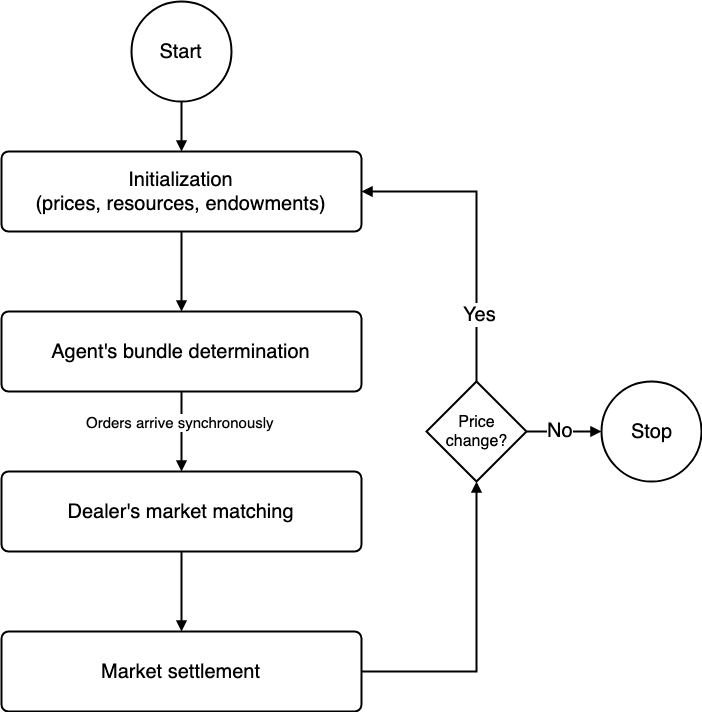
\includegraphics[width=.4\linewidth]{./figures/btm_flowchart.png}
	\caption{Flowchart of the BTM Framework}
	\label{figure:btm_flowchart}
\end{figure}




\begin{comment}

\end{comment}


\section{Concept of LEM Simulation Platform}
\label{sec:concept_of_lem}
To start off, this section brings together the previous sections \ref{sec:about_blockchain} and \ref{sec:btm},
and explains how the BTM and a blockchain interact to implement the BLEMS.
Finally, this section gives an example of a LP in terms of energy efficient demand side management of households. 

First, in the presented BTM in section \ref{sec:btm}, independent, self-interested agents trading bundled resources
in a double-auction market. 
In case of the BLEMS, the agents of the BTM represent households that 
trade independently and self-interested bundles of energy resources to minimize their monetary expense 
through optimally scheduling the operation and energy consumption 
of all energy consuming appliances.

Second, blockchain is introduced as the applied ICT of the BLEMS. 
As already mentioned earlier, the implementation of LEM needs local distributed control and 
management techniques, which can be addressed by the blockchain technology.
This implies that the respective households submit and receive all relevant data, information, and payments via a blockchain. 
Moreover, the double-auction market which enables households to trade their energy bundles is operated by a dealer.
In turn, the dealer is implemented by a smart contract in conjunction with a conventional software client. 
The dealer's smart contract contains all relevant information regarding the market mechanism, like submitted orders, trades, 
dealer's inventory, and market prices. 
Therefore, households exclusively communicate with the dealer's smart contract. 

\begin{figure}[htbp]
    \centering
    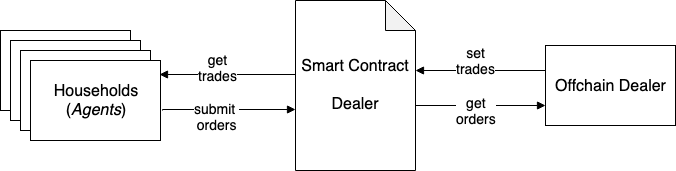
\includegraphics[width=.7\linewidth]{./figures/concept_lem.png}
    \caption{Simplified presentation of the applied communication}
    \label{figure:concept_lem}
\end{figure}

As can be seen in Figure \ref{figure:concept_lem}, the households submit their orders to the dealer's smart contract. 
Afterwards, the dealer's conventional software client, labeled as \textit{off-chain} dealer in the Figure, fetches all existing orders contained in the smart contract
and solves the MMP.
Secondly, the off-chain dealer updates all relevant information in the smart contract, for instance 
the settled orders, the trades, the new market prices, and the resource inventory.
Finally, the households get their respective trades from the dealer's smart contract. 

Anyway, the off-chain dealer is necessary due to the complex and costly calculation of the MMP.
As mentioned in section \ref{sec:transaction}, each transaction consumes gas. Additionally, each mathematical operation in a smart contract
increases the amount of gas to be paid for the respective transaction. As a consequence, implementation and execution of the MMP
in the smart contract itself would be hard to realize and associated with high transaction costs. 

Hence, a well-designed smart contract should move computational complexity off-chain
and focus more on updating state in the contract \shortcite{calculate_cost_eth}. A balance between on-chain
and off-chain complexity should be found.

In addition, we mentioned in section \ref{sec:btm} that the BLEMS applied a synchronous
call market. That means, the dealer only executes the MMP after all agents have submitted their orders.
Likewise, we mentioned in section \ref{sec:smart_contract} that smart contracts are only active and run if they called by a transaction.
They will never run on his own or in the background. For this reason, a mechanism is necessary which triggers the execution of the 
MMP. The implementation of an off-chain dealer is also suitable for this.

So far, this section presented the basic idea and concept of the BLEMS
and explained the necessity of all existing components. In the following section \ref{sec:implementation}, 
the setup and technical implementation is described in detail. 

However, we stated earlier in this section that the agents of the BTM represent households
that trade bundles of energy resources to minimize the monetary expense. 
In section \ref{sec:btm_problem_overview}, we introduced the individual LPs of the agents.
Further, we explained in section \ref{sec:agent_bidding} that a rational agent will choose an improving bundle for 
trading which leaves his wealth level on the same level or better off and defined the selection of such a bundle 
as the BDP.
Finally, to embed the BTM into the topic of LEM, we need to define 
a LP which depicts the energy efficient demand side management of households.

\subsection{Demand Side Management of a Household}
This subsection will embed the BTM into the topic of LEM. 
Therefore, we develop an exemplary and simplified LP in terms of energy efficient demand side management of households. 
That means the objective of the respective households is to minimize their monetary expense regarding energy consumption.
However, the minimization of the costs depends on several constraints.
The sufficient provision of energy must be ensured at all times.


\shortciteA{Chen2013} developed such a LP for demand side management of households, on which the following
presented model is based. 

First, we introduce all relevant variables. Let $a$ denotes an appliance, and $A$ the set of all existing appliances in a household.
In that case, an appliance constitutes energy consuming items, e.g. washers, refrigerators, plug-in hybrid vehicles, etc.
Next, the variable $x_{a}$ denotes the energy consumed by an appliance $a$ to a given point in time. 
Further, each appliance $a \in A$ has a maximum energy level that is defined as rated power and described by $P_{a}$.
Additionally, it exists a limit on the total energy consumed by various appliances of a household. This total energy consumption limit is described by $L_{A}$. In case the total energy consumption limit is exceeded, the power network of the household will be tripped out.
Moreover, a household consumes, on the one hand, solar energy from
\textit{photovoltaic systems (PV)} and on the other hand energy from the electrical grid. 
If households do not consume solar energy directly, they have the opportunity to 
store it in batteries, or export it back to the main power grid if the battery is full.
Let $e_{g}$ denote the energy used from the electrical grid, and $e_{s}$ the energy produced by the PV.
In addition, let $p_{g}$ and $p_{s}$ denote the unit price of the energy from the electrical grid and solar energy.
Furthermore, we describe the solar energy used by all appliances of a household as $y_{s}$, the consumed battery energy 
as $y_{b}$ and the remaining solar energy which is not used by the household appliances and stored in the battery as $z_{b}$.

Finally, we developed the following LP for optimization of the household monetary expense.

\begin{equation}
 \begin{array}{ll@{}ll}
 \text{min} & \displaystyle p_{g} \cdot e_{g} + p_{s} \cdot e_{s} &\\
 \text{s.t.}& \displaystyle \sum\limits_{a \in A}^{} x_{a} \leq L_{A} \\
                    & \displaystyle x_{a} \leq P_{a}, \quad \forall a \in A \\
                    & \displaystyle \sum\limits_{a \in A}^{} x_{a} = y_{s} + y_{b} + e_{g} \\
                    & \displaystyle y_{s} + z_{b} \leq e_{s}
 \end{array}
\end{equation}

\clearpage
In the table below, all applied variables of the developed LP are listed:

\begin{longtable}{c|l}
	\caption{Applied variables in LP for optimization of the household monetary expense} 
	\label{table:applied_variables_lp} 
	\\
	\textbf{Variable} & \textbf{Description} \\
	\hline
    $a$ & energy consuming appliance of household \\
	$A$ & set of all existing energy consuming appliances of household \\
	$x_{a}$ & consumed energy of an appliance $a$ \\
	$P_{a}$ & maximum energy level (rated power) of an appliance $a$ \\
	$L_{A}$ & total energy consumption limit of a household \\
	$e_{g}$ & energy used from the electrical grid \\
	$e_{s}$ & energy produced by PV \\
	$p_{g}$ & unit price of energy from electrical grid \\
	$p_{s}$ & unit price of energy from PV \\
	$y_{s}$ & solar energy used by all appliances of a household \\
	$y_{b}$ & consumed batterie energy by all appliances of a household \\
	$z_{b}$ & remaining unused solar energy stored in the batterie \\
\end{longtable} 

As mentioned earlier,
the objective of the respective households is to minimize
their monetary expense regarding energy consumption.
The term $p_{g} \cdot e_{g}$ denotes the costs for energy from the electrical
grid, whereas the term $p_{s} \cdot e_{s}$ denotes the costs for energy from PV. 

Besides, the first constraint ensures that the total energy consumption of all energy consuming
appliances of a household does not exceed the limit of $L_{A}$. 

Next, the second constraint describes the requirement that the consumed energy
for all existing appliances $a$ in a household is less or equal 
to the respective rated power $P_{a}$.

Further, the third constraint makes sure that the energy consumed by all appliances
of a household is the sum of the energy from the electrical grid, the solar energy from the PV system and the battery energy. This implies if the amount of solar and battery energy is not sufficient to cover the energy consumption of all appliances, external energy from the electrical grid will be used. Therefore, it is ensured that sufficient energy is available at all times.

Finally, the fourth constraint describes that the solar energy produced by the PV system is greater or equal to the sum of the consumed and stored solar energy. 
At times when the battery is fully charged and the energy consumption of the 
appliances are covered by solar energy, it is possible to sell the surplus of 
wasted solar energy.
Referring to the BTM, the first two constraints of the proposed linear
programming model constitutes the independent resources that are managed locally.
The shared resources are represented by 
the energy resources $e_{g}$ and $e_{s}$.
Therefore the respective households trade the following limited bundles.

\[
w=
  \begin{pmatrix}
e_{g} \\
e_{s}
  \end{pmatrix}
\]

Consequently, the objective of the LP is written in matrix-vector notation.

\begin{equation*}
 \begin{array}{ll@{}ll}
        \text{min} & \displaystyle p^{T} \cdot w
 \end{array}
\end{equation*}

where $p^{T}$ denotes the transposed price vector.

\[
p^{T} =
  \begin{pmatrix}
p_{g} &
p_{s}
  \end{pmatrix}
\]



To sum up, this subsection presented a simplified LP for demand side management of a household
that can be integrated into the proposed BTM.

Furthermore, the developed model should only serve as an inspiration and example
and has no claim to completeness. 
It is intended to illustrate how the presented framework can be adapted to enable the trading of energy resources in LEM. 

\clearpage

\section{Implementation}
\label{sec:implementation}

This section outlines the technical implementation of the blockchain-based LEM simulation
and presents parts of the developed source code. Therefore, we give a brief introduction to the applied 
software technologies and present the individual components and their containing attributes and functions.
Finally, we present the simulation process that we divided into \textit{Initial Setup} and \textit{Main Simulation Loop}. 

\subsection{Applied Technologies}
\label{sec:applied_technologies}
In this subsection we give a brief introduction 
to the applied software technologies and libraries.

\paragraph{Python}
An interpreted, object-oriented, high-level programming language with dynamic semantics. 
Additionally, it is simple and comes with an easy to learn syntax \footnote{https://www.python.org/}.
The programming language of choice, which is used to develop the 
respective components that communicate via the blockchain.

\paragraph{Web3.py}
A Python library for interacting with an Ethereum blockchain \footnote{https://github.com/ethereum/web3.py}. 
It enables the developed Python components to communicate via the blockchain.

\paragraph{Ganache}
A personal blockchain for Ethereum development \footnote{https://github.com/trufflesuite/ganache-cli}.
It simulates a full client behavior and makes developing Ethereum applications faster, easier and safer.
Ganache is provided on the one hand as a software tool with a graphical user interface (GUI) and on the other hand as command-line tool (CLI). In the develop LEM simulation the command line version of Ganache is used. 

\paragraph{Solidity}
A statically typed, contract-oriented, high-level programming language for implementing smart contracts on the Ethereum
blockchain \footnote{https://github.com/ethereum/solidity}.
It is used to implement the smart contract dealer. 

\clearpage
%--------------------------------------
\subsection{Components}
\label{sec:components_of_simulation}
We present the three main components \textit{Agent},\textit{Smart Contract Dealer} and \textit{Off-chain Dealer} 
in this subsection and introduce their attributes and functions. 

\subsubsection{Agent}
\label{sec:agent_class}
The agents are implemented by a Python class and the naming is oriented on the proposed BTM.
As stated in section \ref{sec:concept_of_lem}, the agents represent the respective households in the BLEMS. 
First, the class attributes are presented and the associated source code is shown
in the following Listing \ref{lst:agent_class_attributes}.

\begin{lstlisting}[label=lst:agent_class_attributes, caption=Overview of the agent class attributes, language=Python]
    class Agent(object):

    def __init__(self, agent_number, account_address, web3, dealer_contract):
        self._name = 'AGENT{}'.format(agent_number)
        self._account_address = account_address
        self._web3 = web3
        self._dealer_contract = dealer_contract
        self._optimization_problem = None
        self._bundle_set = None
        self._bid = None
        self._mkt_prices = None
        self._trade = None
        self._objective = None
        self._wealth = None
        self._accept_trade = None
\end{lstlisting}

The variables \verb|agent_number|, \verb|account_address|, \verb|web3| and \verb|dealer_contract| are initialized when the class is instantiated.
The variable \verb|agent_number| is used to identify the different agents.
Due to its uniqueness, the \verb|account_address| could be also used as an identifier, 
but it would be cumbersome due to the cryptic hexadecimal representation of the blockchain account addresses.
Therefore a more comprehensible name for each agent is established.
Furthermore, each agent is assigned an Ethereum blockchain account defined by the variable \verb|account_address|. It is required to submit and 
receive transactions via the blockchain.
The Python library for interacting with an Ethereum blockchain is represented by the variable \verb|web3|.
Moreover, the \verb|dealer_contract| constitues an object of the dealer's smart contract that knows all of its implemented functions.
Hence, this variable is needed to call the functions of the smart contract out of this Python class.
All other presented class attributes in the Listing are set during the simulation process.\\

Next, some of the essential functions of the class are introduced and described in detail.

The agents require a function for receiving their optimization problems, which 
implementation is presented in Listing \ref{lst:lp_setter}.

\begin{lstlisting}[label=lst:lp_setter, caption=Setter of optimization problem, language=Python]
    @optimization_problem.setter
    def optimization_problem(self, value):
        self._optimization_problem = value
        self._objective = self._optimization_problem.solve().fun
        self._wealth = self.balance + abs(self._objective)
\end{lstlisting}

After setting the optimization problem, the class attributes \verb|objective| and \verb|wealth| are determined.
In this case, the attribute \verb|wealth| is defined exactly as in the BTM. 
The \verb|balance| constitues the cash endowment $e_{j}$ and \verb|objective| the optimal value of the agents
problem depending on the current amount of the shared resources $z_{j}(c_{j})$.
However, \verb|balance| is not a class attribute, but a class function that uses 
\verb|web3| and \verb|account_address| to retrieve the current
balance of the account from the blockchain.

In addition, the implementation of the function for solving the BDP and hence determining 
the improving bundle set and the associated bid is introduced in the Listing \ref{lst:determine_bundle}.

\begin{lstlisting}[label=lst:determine_bundle, caption=Determining of bundle attributes, language=Python]
    def determine_bundle_attributes(self):
        result = solve_bundle_determination(self._optimization_problem, self._mkt_prices)
        self._bundle_set = result.x
        self._bid = self._objective - result.fun
\end{lstlisting}

First, the BDP is solved in a separate function in subject to the optimization problem and the current market prices.
The associated source code of the function can be found in the appendix \ref{appendix:additional_agent}.

The \verb|bundle_set| constitutes the improving bundle set and is assigned from the results of the BDP.
Further, the \verb|bid| is initialized. We stated that the BTM implemented nonstrategic bidding and pricing,
wherefore an agent always submits a limit price equal to the valuation of the bundle, such that $l(w) = v(w)$.
The value of \verb|bid| is assigned by the difference of the \verb|objective| $z_{j}(c_{j})$ and the 
objective of the optimization problem with the additional resources of the \verb|bundle_set| $z_{j}(c_{j}+w)$, 
which reflects the definition of the bundles true value $v(w) = z_{j}(c_{j}) - z_{j}(c_{j}+w)$.

Next, Listing \ref{lst:set_order} presents the implementation of the function for 
submitting orders to the dealer's smart contract.
Currently, smart contracts in Ethereum do not fully 
support fixed point numbers. It is possible to declare them, but they cannot be assigned to or from \shortcite{solidity_fixed_point}.
This poses a problem because the values in the BTM often contain fixed point numbers. Therefore, 
we developed a workaround that shifts the decimal places to the right and truncates
the remainder when values sent to the dealer's smart contract so that integer values are generated.
When obtaining values from the dealer's smart contract we shift the decimal places to the left to restore 
the original fixed point values. 
Due to this, the \verb|bundle_set| and \verb|bid| are prepared for 
sending to the dealer's smart contract.

\begin{lstlisting}[float=htbp, label=lst:set_order, caption=Submitting of order, language=Python]
    def set_order(self):
        bundle_set = utils.prepare_for_sending(self._bundle_set)
        bid = utils.prepare_for_sending(self._bid)
        
        if(bid > 0):
            prepayment = utils.from_ether_to_wei(self._bid)
        else:
            prepayment = 0

        self._dealer_contract.contract.functions.setOrder(bundle_set, bid, prepayment).transact({'from': self._account_address, 'value': prepayment})
\end{lstlisting}

Additionally, it is identified if the \verb|bid| represents a buy or a sell order by examining if the value 
of \verb|bid| is greater than zero. In case of a buy order, the agents have to pay in advance, to which 
the variable \verb|prepayment| is assigned in the amount of \verb|bid|.
We implemented this procedure to prevent the strategic placing of orders and to ensure 
that the financial resources are available.
In case of a sell order, no payment in advance is required and the \verb|prepayment| is set to zero.
Moreover, Wei is a subdivision of the cryptographic currency of Ethereum and presents the base unit within smart contracts.
As 1 Ether is defined as $10^{-18}$ Wei, we decided to specify all monetary values on the side 
of the agents and the off-chain dealer in Ether for better clarity.
Therefore, the \verb|bid| is converted from Ether to Wei before assigning to the \verb|prepayment|.
Finally, the \verb|dealer_contract| is used to call the function of the dealer's smart contract which is
responsible for setting the orders.

Moving calculations off the blockchain comes along with the drawback that source code is not
transparent to all agents anymore. 
That comes to bear in the opacity of the trade calculation of the dealer. 
To adress this issue we implemented a trade verification procedure based on 
strong duality theory, which implementation is outlined in Listing \ref{lst:verify_trade}.
The verification procedure applies the Strong Duality Theorem to verify the validity of the off-chain dealer's calculations.
That means, if the primal MMP has an optimal solution $x^{*}$, then 
the dual also has an optimal solution $y^{*}$, such that $c^{T}x^{*} = b^{T}y^{*}$.
Due to this, it is possible to verify if the solution of the dealer is optimal, without solving the corresponding MMP. 
The agents calculate whether strong duality holds and decide on the basis of the result whether they accept the trade or not.
Because of the limitations of floating point arithmetic \footnote{https://docs.python.org/2/tutorial/floatingpoint.html}, 
we round off the values of the MMP and the dual problem to make sure that correct trades 
are not rejected based on limited machine accuracy.
Finally, the class variable \verb|accept_trade| is assigned according to the result of the trade verification 
procedure.

\begin{lstlisting}[float=htbp, label=lst:verify_trade, caption=Verification of trades, language=Python]
    def verify_strong_duality(self):
        mmp_values, mmp_duals, mmp_target_coefs, mmp_bounds = self.get_mmp_attributes()
        primal_solution = (-np.sum(mmp_values * mmp_target_coefs))
        dual_solution = np.sum(mmp_duals * mmp_bounds)
        primal_solution = math.floor(primal_solution * 10) / 10
        dual_solution = math.floor(dual_solution * 10) / 10

        if primal_solution == dual_solution:
            self._accept_trade = True
        else:
            self._accept_trade = False
\end{lstlisting}


Likewise, the class contains a function for notifing the dealer's smart contract if the respective trade is accepted or not,
as shown in the Listing \ref{lst:accept_trade}.

\begin{lstlisting}[float=htbp, label=lst:accept_trade, caption=Notification of trade acceptance, language=Python]
    def accept_trade(self):
        if(self._accept_trade):
            trade = self._dealer_contract.contract.functions.acceptTrade(self._accept_trade).call({'from': self._account_address})
            self._trade = utils.prepare_for_storing(trade)

        self._dealer_contract.contract.functions.acceptTrade(self._accept_trade).transact({'from': self._account_address})

\end{lstlisting}

In case the trade is accepted, it is fetched and stored in the variable \verb|trade|. Since the trade 
is fetched from the dealer's smart contract, the stated workaround that shifts the decimal places follows
at this point to restore the original fixed point values.
Furthermore, an almost identical function invocation of the dealer's smart contract 
function \verb|acceptTrade()| is indicated twice. 
The difference lies in the methods \verb|call()| and \verb|transact()|. 
The \verb|call()| method enables to invoke any smart contract function on a read-only basis
and returns values sent by the smart contract return statement. 
Those read-only invocations run much faster than transactions that require network verification.
On the contrary, the \verb|transact()| method submits a verified transaction that potentially changes the state of the blockchain. 
Hence, network verification is needed that causes a significant delay due to the mining procedure.
Consequently, this method does not return the values of the smart contract return statements,
but the transaction hash of the submitted verified transaction.
Regarding the implementation, the first invocation only serves to fetch the respective trade,
whereas the second call of the function serves to notify the dealer whether the trade has been accepted or not.
For this reason, the first call of the dealer's smart contract function \verb|acceptTrade()| 
is only executed if the trade is accepted. 

Finally, the implementation of the function for adding the received trade to the shared resources is presented 
in Listing \ref{lst:add_trade_to_shared_resources}.

\begin{lstlisting}[float=htbp, label=lst:add_trade_to_shared_resources, caption=Adding of trade to shared resources, language=Python]
    def add_trade_to_shared_resources(self):
        if(self._accept_trade):
            self._optimization_problem.shared_resources = np.add(self._optimization_problem.shared_resources, self._trade)
            self._objective = self._optimization_problem.solve().fun  
            self._wealth = self.balance + abs(self._objective)
\end{lstlisting}

The body of the function is only executed if the trade has been accepted.
First, the new allocation of the shared resources is calculated ($c_{j} \leftarrow c_{j} + w_{j}^{*}$).
Due to the new allocation of shared resources, the \verb|objective| and also the \verb|wealth| is recalculated accordingly.


\subsubsection{Smart Contract Dealer}
\label{sec:smart_contract_dealer}
The smart contract dealer is implemented by the programming language Solidity, which is the most popular and frequently 
used language for Ethereum smart contracts. In the beginning, the attributes are outlined and presented in Listing 
\ref{lst:contract_attributes}.

\begin{lstlisting}[float=htbp, label=lst:contract_attributes, caption=Attributes of Smart Contract, language=Java]
    contract Dealer{
        // general attributes
        address private _owner;
        int256[] public resource_inventory;
        int256[] public mkt_prices;

        // attributes for order management
        uint32 public order_count;
        uint32[] public order_indices;
        mapping(uint32 => Order) public orders;

        // attributes for trade management
        mapping (address => uint256) account_index; 
        address[] public trades_accounts;
        mapping(address => int256[]) public trades;
        mapping(address => uint256) public bills;
        mapping(address => uint256) public prepayments;
        mapping(address => uint256) public refunds;
\end{lstlisting}

First, general attributes are declared, to which the attributes \verb|owner| belongs.
We stated that the creator of a smart contract does not have any special permissions at the protocol level, but
that it is possible to specify explicitly those special permissions in the source code.  
For this reason we initialized this variable with the address of the contract creator, who is, in our case,
the off-chain dealer. The \verb|owner| comes to bear in the implementation of the modifier \verb|onlyByOwner()|.
A modifier can be seen as an extension of a function and is mainly used to 
to check if certain conditions are met before executing the rest of the source code in the body of a function.
We have built the modifier to ensure that only the owner of the contract has the authority to perform certain functions.
In addition, attributes for managing the orders and trades of the agents are declared. 
The orders, trades and additional properties of the trades are predominantly managed in mappings.
A mapping is a collection of key-value pairs, in which all keys and all values must be of the same 
data type. However, Solidity does not provide an iteration
function to retrieve all the lists that are stored in a mapping, wherefore it is not possible 
to read the values from the mapping without knowing the respective keys.
Therefore, we developed a workaround and store the keys of mappings in additional arrays which serves 
as look up tables.
With reference to the Listing \ref{lst:contract_attributes}, the array \verb|order_indices| functions as a 
look up table for the mapping \verb|orders|, and the array \verb|trades_accounts| for the mapping 
\verb|trades| and all other trades related mappings. \\

Next, the essential functions of the dealer's smart contract are introduced and described in detail.

The function for receiving the orders of the agents is outlined in the Listing \ref{lst:set_order_contract}.
It contains, on the one hand, the Solidity built-in modifier \verb|payable|, and on the other hand, the custom
modifier \verb|checkPrepayment|. To allow a function to receive payments, it must be declared as \verb|payable|,
otherwise the incoming payment would not be accepted and the belonging transaction would not terminate successfully.
In order to receive the prepayments of the agents, this function requires the stated modifier.
Further, we developed the second modifier \verb|checkPrepayment|, which checks whether the amount sent with the 
transaction corresponds to the amount to be paid. Thus it is verified if the transaction is a valid order.
Hence, if the prepayment is not sufficient, the function call of the agents is rejected and 
the order is not accepted.


\begin{lstlisting}[float=htbp, label=lst:set_order_contract, caption=Receiving agents orders, language=Java]
    function setOrder(int256[] _bundle, uint256 _bid, uint256 _prepayment) public payable checkPrepayment(_prepayment) {

        Order memory new_order = Order(
            msg.sender,
            _bundle,
            _bid
        );
        orders[order_count] = new_order;
        order_indices.push(order_count);

        // increment order count
        order_count ++;
    }
\end{lstlisting}

If the preconditions defined by the modifiers are fulfilled and the function body is executed, 
the variable \verb|new_order| is initialized by the object \verb|Order|. The object is implemented by the data type
struct, which is a user-defined data container for grouping variables and is well suited to bundle and 
manage all necessary information regarding the orders. The \verb|msg.sender|, \verb|bundle| and \verb|bid|
are contained in the data container and represent the essential information regarding an agents order.
When a contract is executed, it has access to a small set of global objects to which the object \verb|msg| belongs.
This object contains information regarding the transaction which invokes the contract execution,
such as the account address that can be accessed by the variable \verb|msg.sender|.
Finally, the \verb|new_order| is added to the mapping \verb|orders|, to which 
the incremental number \verb|order_count| serves as the key.
After each incoming order, the number is increased by one and added to the array \verb|oder_indices|
that serves as a look up table as mentioned earlier.

Furthermore, the function which serves to set the trades of the agents is introduced in Listing \ref{lst:set_trade_contract}.
With reference to the function header, the modifier \verb|onlyByOwner()| is applied, which ensures that
only the owner of the contract has the authority to call this function
It is required, since nobody except the owner (off-chain dealer) should have 
the permission to call this function and thus to set the trades of the agents.

\begin{lstlisting}[float=htbp, label=lst:set_trade_contract, caption=Setting the trades, language=Java]
    function setTrade(address _account, int256[] _trade, uint256 _prepayment, uint256 _bill, uint256 _refund) public onlyByOwner() {
        addToArray(_account);
        trades[_account] = _trade;
        bills[_account] = _bill;
        prepayments[_account] = _prepayment;
        refunds[_account] = _refund;
    }
\end{lstlisting}

Next, the function \verb|addToArray()| is called, which examines whether the belonging account 
to a trade is already contained in the array \verb|trades_account|.
If not, the account is added to the array, which again serves as the look up table for the
mapping \verb|trades| and all other trades related mappings. 
Concluding, all the required information for a trade are placed in the corresponding mappings, 
in which the account address is used as the key.

In the end, a last function of the dealer's smart contract is introduced.
The implementation of the function is shown in Listing \ref{lst:accept_trade_contract} above
and can be seen as a kind of collection point for the trades.

Finally, the function for providing the trades of the agents is outlined and shown in Listing \ref{lst:accept_trade_contract}.
It can be seen as the interface of trades, as it enables agents 
to accept and fetch or to reject their trades.

\begin{lstlisting}[float=htbp, label=lst:accept_trade_contract, caption=Interface of trades, language=Java]
    function acceptTrade(bool accept_trade) public returns (int256[]) {
        if(accept_trade) {
            msg.sender.transfer(refunds[msg.sender]);
            return trades[msg.sender];
        } else {
            msg.sender.transfer(prepayments[msg.sender]);
            delete trades[msg.sender];
        }
    }
\end{lstlisting}

In case of trade acceptance, the trade is returned and 
the refund is paid to the respective agent who invokes the function. 
As stated, the agents have to prepay the true value of the
requested bundle, but they often only get shares of their requested bundles due
to the solution of the MMP.
For this reason, the agents have often prepaid more than they have to pay, which leads to 
excess payments. Because of this, the dealer calculates the difference between the prepayment 
and the price of the granted trade and refunds it.
In case of a rejection, the dealer refunds the whole prepayment and deletes the granted trade.
The deletion of a rejected trade is necessary to calculate the dealer's resource inventory correctly
after the settlement process.


\subsubsection{Off-chain Dealer}
\label{sec:off_chain_component}
The dealer is implemented by a smart contract in conjunction with 
a conventional software client. In the previous subsection we introduced 
the implementation of the smart contract, so this subsection introduces
the implementation of the conventional software client denoted as 
off-chain dealer. It is implemented by a Python class and its class 
attributes are presented in Listing \ref{lst:offchain_class_attributes}.

Similar to the implementation of the agents, the \verb|account_address|, \verb|web3|, 
\verb|dealer_contract| are initialized by instantiation of the class and serve for 
the same purpose. Besides, the attributes \verb|shared_resource_size| and \verb|mkt_prices|
are initialized simultaneously. The \verb|shared_resource_size| constitutes the amount 
of the various shared resources $c$ and is required to determine the vector size 
of the traded bundles and related market price vector. 
The \verb|mkt_prices| represents the market price vector and is initialized by zeros with subject to
the \verb|shared_resource_size|. The other shown class attributes in the Listing are set during the
simulation process.

\begin{lstlisting}[float=htbp, label=lst:offchain_class_attributes, caption=Overview of the off-chain dealer's class attributes, language=Python]
    class Dealer(object):

        def __init__(self, account_address, web3, dealer_contract, shared_resource_size):
            self._account_address = account_address
            self._web3 = web3
            self._dealer_contract = dealer_contract
            self._resource_inventory = None
            self._trade = None
            self._shared_resource_size = shared_resource_size
            self._mkt_prices = np.zeros(self._shared_resource_size)
            self._order_handler = None
\end{lstlisting}

Next, the essential functions of the class are introduced and explained in detail.
To begin with, the function to retrieve the orders of the agents from the dealer's 
smart contract is introduced in the Listing \ref{lst:offchain_get_orders}.

\begin{lstlisting}[float=htbp, label=lst:offchain_get_orders, caption=Retrievement of orders, language=Python]
    def get_orders(self):
        self._order_handler = utils.OrderHandler()
        order_indices = self.get_order_indices()

        # get all orders from contract and store in order handler
        for order_id in order_indices:
            order = self._dealer_contract.contract.functions.getOrder(order_id).call()
            self._order_handler.add_order(order_id, order)
\end{lstlisting}

We developed a class \verb|OrderHandler| to store and manage the orders of the agents' more easily
on the side of the off-chain dealer. 
It works like a kind of dictionary and contains the account addresses as the key 
and the corresponding trades as values, but additionally provides methods to calculate
the relevant attributes of the trades in subject to the belonging orders.
Therefore, the variable \verb|order_handler| is initialized with an object of this class
and the iteratively retrieved orders from the dealer's smart contract are stored in it.

Furthermore, the class also provides functions for creating and solving the MMP.
Due to the focus on the architectural design and implementation of the simulation and the high complexity
of these functions, they are not presented in detail. However, the corresponding source code can be found in the appendix \ref{appendix:additional_offchain}.

Finally, the function to set the trades of the agents in the dealer's smart contract 
is outlined and presented in the Listing \ref{lst:offchain_set_trades}.
The results from the MMP represent the share of the respective orders and are set for 
each order in the \verb|order_handler|. Then, the calculation of the relevant attributes of the trades
(prepayment, bill, and refund) is executed, wherefore the provided methods of the \verb|OrderHandler| come to bear.

\begin{lstlisting}[float=htbp, label=lst:offchain_set_trades, caption=Submitment of trades, language=Python]
    def set_trades(self):
        self.set_trade_share()
        self.initiate_trade_calculation()
        self.initiate_prepayment_calculation()
        self.initiate_bill_calculation()
        self.initiate_refund_calculation()

        for order in self._order_handler.get_all_orders():
            account, trade, prepayment, bill, refund = order.get_trade_information()
            prepayment = utils.from_ether_to_wei(prepayment)
            bill = utils.from_ether_to_wei(bill)
            refund = utils.from_ether_to_wei(refund)

            self._dealer_contract.contract.functions.setTrade(account, trade, prepayment, bill, refund).transact({'from': self._account_address})
\end{lstlisting}

Concluding, the calculated trades and the corresponding attributes are set iteratively in the dealer's smart contract. 
Again, the monetary values like \verb|prepayment|, \verb|bill|, and \verb|refund| are converted from Ether to Wei and 
the values of the trades are converted to integer by shifting the decimal places.

\subsubsection{Blockchain}
The applied blockchain is described in this subsection. In section \ref{sec:applied_technologies}, we already
stated that we used a personal blockchain called Ganache, which acts like a personal Ethereum full client  
However, Ganache provides even more features that allow you to customize the properties of the Blockchain.
First, you can specify the number of generated accounts and the assigned amount of ether.
This is a proper way to specify the initial cash endowments of the agents ($e_{j},$ for $j=1, ..., k$)
and the dealer ($e_{0}$).
Further, it is possible to adjust the block time, which defines the time it takes to mine a new block. 
Additionally, it provides the feature to instantly mine a new block for every transaction. 
This is very useful for testing and debugging applications like the BLEMS.
Likewise, it is possible to specify the price of gas in Wei and the gas limit of a block. 
Hence, the applied blockchain Ganache allows you to recreate many scenarios of different blockchain behavior
and is therefore perfectly suited for the application of a simulation.


\subsection{Simulation Process}
To begin with, this subsection presents the whole simulation process. 
In contrast to the previous subsection \ref{sec:components_of_simulation}, that 
considered the individual components in isolation, this subsection focus 
on the interaction of the various components.

Further, we divided the simulation process into 
the two parts \textit{Initial Setup}, and \textit{Main simulation loop},
which are described in the following.

\subsubsection{Initial Setup}
Above all, the initial setup part is shown in the Listing \ref{lst:initial_setup}.
The displayed source code is executed directly before the source code from listing \ref{lst:main_simulation_loop}.

\begin{lstlisting}[float=htbp, label=lst:initial_setup, caption=Initial setup of the simulation, language=Python]
    # general setup of simulation
    var = mem.Variables()
    lp.decompose(var)

    # set initial inventory and market prices
    var.dealer.set_resource_inventory()
    var.dealer.set_mkt_prices()  
\end{lstlisting}

Firstly, an object of the class \verb|Variables| is instantiated. 
This class object can be seen as a kind of global memory.
It contains all fundamental variables which are required to run the simulation.
These variables are described in more detail in the following list.

\begin{description}
	\item[\texttt{central\_problem}:] Represents the specified central optimization problem of the presented BTM.
    It is divided into subproblems and distributed to the existing agents. It is important 
    to note that the number of variables present in the problem can be exactly divided by the number of agents.
    Otherwise, an exception is thrown.
	\item[\texttt{web3}:] Represents the object of the Python library, which enables the interaction with an
	Ethereum blockchain. It is the same object that is passed to the agent classes and the off-chain dealer class.
    \item[\texttt{dealer\_contract}:] Represents the object of the dealer's smart contract. 
    It is the same object that is passed to the agent classes and the off-chain dealer class. It contains all the
    implemented functions of the dealer's smart contract. When the contract is deployed and thus anchored in the blockchain, a JSON file is created. 
    This file is denoted as the \textit{Contract Application Binary Interface (ABI)}. The ABI is used to instantiate the Python object.  
    \item[\texttt{agent\_pool}:] Represents a list containing all existing agent objects. 
    Therefore all existing accounts are read from the blockchain and used to instantiate the agents.
    \item[\texttt{dealer}:] Represents the object of the off-chain dealer, which is instantiated with the 
    remaining account.
\end{description}

Next, the function for decomposing the central problem is called. The class object \verb|Variables| is passed to it as a parameter.
This is needed to reach the central problem, the agent pool and thus the amount of all existing agents, and the object of the
off-chain dealer. 
Then, the central problem is decomposed into subproblems which are distributed among the agents. 
The distribution step also includes the distribution of the shared resources. 
Further, the allocation of the shared resources is implemented in such a way that all parties receive equal shares.

Furthermore, the off-chain dealer sets the initial values of the resource inventory and the market prices in the dealer's
smart contract. As stated before, the initial resource inventory is calculated in the decomposition step of the central problem. 
We also mentioned earlier in \ref{sec:off_chain_component}, that the market price vector is initialized when instantiating the off-chain dealer class.
The size of the market price vector is equal to the size of the shared resources and is initially specified with zeros.

Finally, a few simulation parameters are set, which are needed to determine the termination of the simulation.
These are self-explanatory and not essential for understanding the simulation process, wherefore they are not shown in the Listing \ref{lst:initial_setup}.
Afterwards, the main simulation begins.

\subsubsection{Main Simulation Loop}
First of all, the source code of the \textit{Main simulation loop} is outlined in the Listing \ref{lst:main_simulation_loop}.
These loop represents the main process of the simulation and takes place after the part \textit{Initial Setup}.
The simulation loop is implemented by a while loop, which only terminates if the 
market prices from the previous round are equal to the market prices of the current round.
Conversely, this means that the simulation runs as long as the market prices of the last two rounds are different.
Additionally, there are comments in the source code of Listing \ref{lst:main_simulation_loop}.
The inline comments to the right of the function calls indicate if the invoked function constitutes
a \verb|call()| or a \verb|transact()| method. As described earlier, the \verb|call()| method invokes 
a smart contract function on a read-only basis, whereas the \verb|transact()| method submits a verified transaction 
that changes the state of the blockchain.

\begin{lstlisting}[float=htbp, label=lst:main_simulation_loop, caption=Main loop of the simulation, language=Python]
    while(not equal_market_prices):
        
        # agent bidding
        for agent in var.agent_pool:
            agent.get_mkt_prices()  # call
            agent.determine_bundle_attributes()
            agent.set_order()  # transact

        utils.wait_for_new_block(var)

        # dealers market matching mechanism
        var.dealer.get_orders()  # call
        var.dealer.create_mmp()
        var.dealer.solve_mmp()
        var.dealer.set_trades()  # transact
        var.dealer.delete_order()  # transact
        var.dealer.set_mkt_prices()  # transact
        var.dealer.set_mmp_attributes()  # transact

        utils.wait_for_new_block(var)

        # agent trade verification
        for agent in var.agent_pool:
            agent.verify_strong_duality()  # call
            agent.accept_trade()  # transact
            agent.add_trade_to_shared_resources()

        utils.wait_for_new_block(var)

        var.dealer.recalculate_resource_inventory() # transact        
\end{lstlisting}

The behavior of a blockchain differs from that of conventional client-server architecture.
In a blockchain environment, the process of a \verb|transact()| method call is not immediately completed.
The network verification requires some time due to the mining procedure. 
Consequently, before the values written into the blockchain by a \verb|transact()| method are accessible, a certain time passes.
Hence, it is important to take this into account if you want to read certain values 
from the blockchain that you set in previous steps. 
Therefore, we implemented a function called \verb|wait_for_new_block()|. This function
simply waits for the generation (mining) of a new block and 
is invoked whenever it is needed to wait for new values to be finally anchored in the blockchain.

In addition, the \textit{Main simulation loop} can be divided into the three main activities 
\textit{agent bidding}, \textit{dealer's market matching mechanism}, and \textit{agent trade verification},
which are also marked with a comment in the Listing \ref{lst:main_simulation_loop}.
These main activities are thematically summarised function calls.
Besides, the above described function \verb|wait_for_new_block()| is called between these activities
to ensure a faultless process. 
In the following, each of the three activities is described.

\paragraph{Agent bidding:}
To start with, this activity refers to section \ref{sec:agent_bidding} of the same name and represents
the technical implementation. Further, a sequence of all function 
calls for this activity is provided in Figure \ref{figure:agent_bidding_figure}.

Above all, the steps described below are performed for all existing agents. 
This is indicated by the specified for-loop, shown at the beginning of Listing \ref{lst:main_simulation_loop}.

\begin{figure}[htbp]
	\centering
	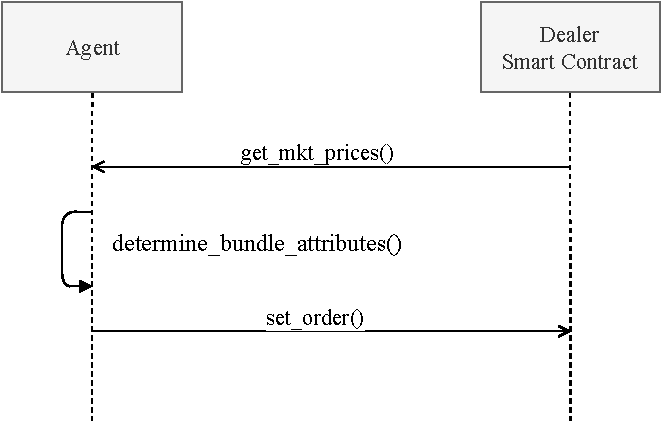
\includegraphics[width=.8\linewidth]{./figures/agent_bidding.pdf}
	\caption{Sequence of agent bidding}
	\label{figure:agent_bidding_figure}
\end{figure}

First, the agent gets the current market prices from the dealer's smart contract.
To obtain the market prices, the function \verb|getMktPrices()| of the dealer's smart contract is utilized.
The market prices are required for the determination of the preferred bundle set.

Next, the agent solves the bundle determination and initialize the class attributes
\verb|bundle_set| and \verb|bid|.
In turn, they are required for the next function call.
The corresponding implementation of this function is presented in Listing \ref{lst:determine_bundle}.

Finally, the agent sets the order in the dealer's smart contract.
To place the order in the contract, the function \verb|setOrder()| of the contract is utilized.
The implementation of the dealer's smart contract function is shown in the Listing \ref{lst:set_order_contract}.
Moreover, the implementation of the function \verb|set_order()| of the agent is 
also introduced in the Listing \ref{lst:set_order}.

\paragraph{Dealer's market clearing mechanism:}
To begin with, this activity refers to section \ref{sec:market_clearing_mechanism} and can be seen as
the technical implementation. Further, a sequence of all function 
calls for this activity is provided in Figure \ref{figure:dealers_mmp}.

First, the off-chain dealer gets the orders from the dealer's smart contract.
Therefore, the function \verb|get_orders()| of the agent (introduced in Listing \ref{lst:offchain_get_orders})
utilizes the function \verb|getOrder()| of the contract.

Then, the off-chain dealer creates and solves the MMP.
The implementation of both functions is outlined in appendix \ref{appendix:additional_offchain}.

\begin{figure}[htbp]
	\centering
	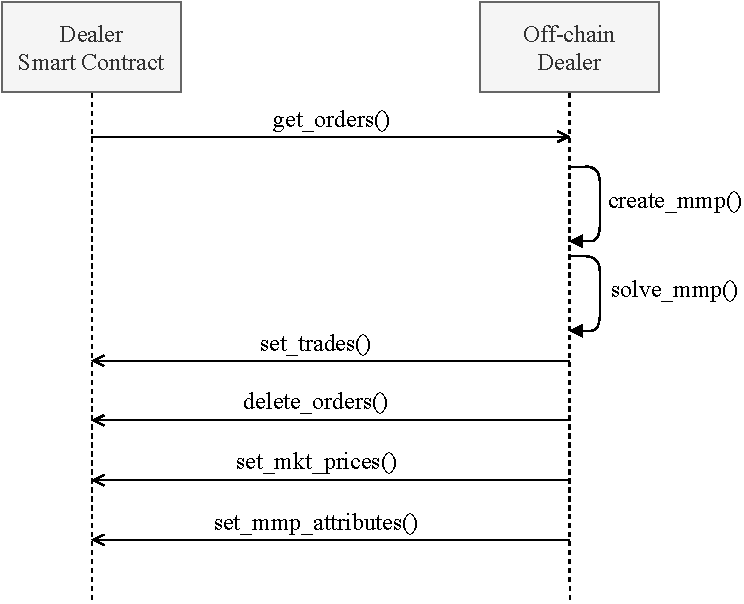
\includegraphics[width=.8\linewidth]{./figures/dealers_mmp.pdf}
	\caption{Sequence of dealer's market matching mechanism}
	\label{figure:dealers_mmp}
\end{figure}

After solving the MMP and the calculation of the respective 
trades, the off-chain dealer sets the trades in the dealer's smart contract.
Therefore, the function \verb|set_trade()| of the off-chain dealer (introduced in Listing \ref{lst:offchain_set_trades})
utilizes the function \verb|setTrade()| of the dealer's smart contract.

Afterwards, the off-chain dealer deletes the settled orders out of the dealer's
smart contract. 
To do this, the function \verb|delete_order()| of the off-chain dealer
utilizes the function \verb|deleteOrder()| of the dealer's smart contract.

In addition, the off-chain dealer sets the new market prices in the dealer's smart contract.
To set the new market prices, the function \verb|set_mkt_prices()| of the off-chain dealer 
utilizes the function \verb|setMktPrices()| of the dealer's smart contract.

Finally, the values of the MMP are set in the dealer's smart contract. 
They are used by the agents to verify the correctness of the calculated market prices.
Therefore, the function \verb|set_mmp_attributes()| of the off-chain dealer
utilizes the function \verb|setMMPAttributes()| of the dealer's smart contract.

\paragraph{Agent trade verification:}
To start, this activity covers the entire trade verification step of the agent. 
Likewise, a sequence of all function 
calls for this activity is provided in Figure \ref{figure:agents_trade_verification}.

\begin{figure}[htbp]
	\centering
	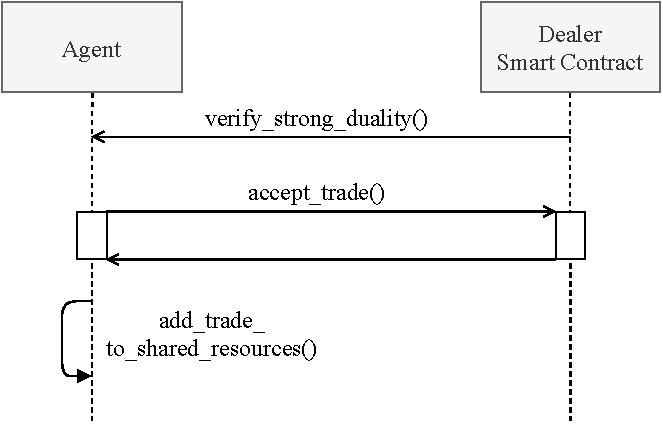
\includegraphics[width=.8\linewidth]{./figures/trade_verification.pdf}
	\caption{Sequence of agents trade verification}
	\label{figure:agents_trade_verification}
\end{figure}

First, the agent verifies if the conditions of the Strong Duality Theorem
are fulfilled.
Therefore, the function \verb|verify_strong_duality()| of the agent
(introduced in Listing \ref{lst:verify_trade})
utilizes the function \verb|getMMPAttributes()| of the dealer's smart contract.
As mentioned ealier in section \ref{sec:agent_bidding}, this function 
determine the class variable \verb|accept_trade| of type Boolean,
which indicates whether the trade is accepted or not.

Afer that, the agent informs the dealer's smart contract whether 
the trade is accepted or rejected.
For this, the function \verb|accept_trade()| of the agent
(introduced in Listing \ref{lst:accept_trade})
utilizes the function \verb|acceptTrade()| of the dealer's smart contract
(introduced in Listing \ref{lst:accept_trade_contract}).
In case of acceptance, the dealer's smart contract transfers the refunds 
to the agents and returns the respective bundle. Otherwise, in case of  
rejection, dealer's smart contract transfer the whole prepayment 
and deletes the respective trade.

Finally, the agent adds the trade to the shared resources. The invocation
of this function only affects if the trade was previously accepted. \newline

At the end of each iteration, the resource inventory of the dealer is recalculated.
Therefore the off-chain dealer calculates how much of the inventory is used for
the trades and settles this with the previous inventory.
Finally, the new calculated inventory is set in the dealer's smart contract.

\clearpage

\section{Conclusion}
In this research, we described the difficulties of integrating distributes renewable energy sources (RES) into 
the existing electric grid and presented peer-to-peer (P2P) energy trading in local energy markets (LEM)
as a possible solution to technical and market problems. Further, we pointed out that central
management in P2P energy trading is challenging due to the need for advanced communication and data exchanges,
wherefore local distributed control and management techniques are more suitable.
Therefore, we introduced the Ethereum-based blockchain as a new and innovative information communication technology (ICT), 
which fulfills the need for distributed control and management techniques.
Moreover, we presented the Bundle Trading Market Framework (BTM), which solves a distributed system
optimization problem by self-interested agents that iteratively trading bundled resources in a double
auction market run by a dealer. 
Then, we brought all introduced topics together and proposed a concept for an open blockchain-based 
LEM simulation (BLEMS). Therefore, we presented the architectural design and embedded the BTM into the topic of LEM
by conceptualizing a linear program (LP) for demand side management of households. 
Finally, the technical implementation of the BLEMS is outlined, in which we described the issues due to
specific properties of blockchain and presented the applied solutions.

In the following section, we investigate whether the developed simulation contains all components for the efficient 
operation of a blockchain-based LEM, which are introduced in section \ref{sec:components_of_local_energy_markets}. 
Then, we outline the contribution of this research. Finally, we examine further areas of research.

\subsection{Compliance of LEM Components}
\label{sec:compliance_of_components}

In this subsection, we examine if the seven components for the efficient operation of LEM,
elaborated by \shortcite{mengelkamp2018designing}, can be 
provided by the developed simulation platform.
Referring to the microgrid setup (C1), an explicit objective, a definition of the market participants and a definition of the form of the traded energy is required. The developed simulation can meet these requirements. The explicit objective can be defined by the researcher itself by setting up a central problem. It is possible to define the market participants and the form of the traded energy bundles
according to your requirements.
Referring to the grid connection (C2), well defined connection points to the superordinate main grid are required.
These connection points are not implemented yet, but the implementation of these connection points 
into dealer's smart contract is possible.
It would be conceivable to integrate these into the inventory policy of the dealer.
As for the information system (C3), the requirements are fulfilled due to the usage of blockchain as the ICT.
Moreover, the applied BTM constitutes an appropriate market mechanism (C4). The BTM defines a clear bidding strategy and the 
overall objective of the applied framework is to provide an optimal allocation in near real-time. 
Additionally, the BTM determines the respective prices by calculating the dual variables.
Therefore, the developed simulation also includes a pricing mechanism (C5) that supports an efficient allocation.
Likewise, a suitable EMTS (C6) is provided by the applied BTM. 
It ensures automatically the energy supply and aims to minimize energy costs.
Finally, the developed simulation lacks the definition of how LEM fit into the current energy policy and how taxes and fees are distributed and billed. 
That is why the component regulation (C7) is not fulfilled. 
In conclusion, the developed simulation provides five of seven components for the efficient operation of LEM. 
Besides, it allows the integration of the missing two components.
Therefore, the BLEMS provides an appropriate and valuable basis for a substantial and significant simulation of LEM. 

\subsection{Contribution}
The conducted research provides two core contributions.

First, the decentralized implementation of the proposed BTM. 
We successfully implemented the BTM with a blockchain as the applied ICT, 
as the sum of the agents objectives equals the objective of the central problem. 
We also applied the numerical example of \shortciteA{guo2007market} and 
ended up with the same objectives and resource allocations, listed in the log 
of the executed simulation in appendix \ref{appendix:log_output}.
Since the application of blockchain technology, the technical implementation
is publicly accessible, wherefore more transparency is provided and the 
required level of trust in the BTM is reduced. 
Nevertheless, to increase efficiency of the distributed solution,
we moved calculations off-chain, wherefore the respective source code 
is not transparent to all stakeholders anymore.
To address this issue, we developed the \textit{Agent Trade Verification} procedure,
which based on strong duality theory.
Therefore, the level of transparency is maintained and
the appliance of commercial solvers is enabled. 
Additionally, the blockchain contains cryptographic encryption methods,
which also raises the level of security in the BTM.
In conclusion, a secure and decentralized market-based optimization algorithm for distributed systems has 
been developed.

Second, we conceptualized a LEM simulation based on the implemented
BTM. We proposed an exemplary linear programming problem in terms of 
energy efficient demand side management of households to embed the BTM into the topic of LEM.
Moreover, the conducted research removes technical barriers.
The section \ref{sec:implementation} provides a detailed 
explanation of the implementation and deals with the special features 
of the blockchain functionality.
Hence, the usage of complex distributed ledger technologies (DLT) for researchers
is simplified. 
In addition, the programming language Python is very 
friendly for beginners and eases the entry into the use of the BLEMS.
Therefore, it incentivizes researchers 
to design and test their artifacts by using the BLEMS.
Furthermore, due to the customizability of the blockchain properties 
the developed simulation allows for testing different scenarios and thus 
to get a better understanding of the dynamics of a decentralized LEM.

\subsection{Future Work}
The conducted research offers the potential for future work in many areas.

First, we stated in section \ref{sec:market_clearing_mechanism}, that we
applied a synchronous call market, where submitted orders to the system
will be accumulated and processed simultaneously at periodic intervals.
In a real-world application, it would be more appropriate to clear the market every time new orders arrive. Therefore,
the implementation from the synchronous to the introduced asynchronous market trading environment of \shortciteA{guo2012computational} would be reasonable. 

Second, the implementation of an auction mechanism by a blockchain causes 
difficulties regarding privacy. Every on-chain data is publicly available. 
In case of an auction mechanism, this can result in competitive advantages
for those who submit their orders later on. 
In an environment where all orders submitted simultaneously and written into the same block, this would not be an issue. 
Otherwise, in an environment where orders submitted at different times and written into different blocks,
some participants will have a competitive advantage, as they can see the orders 
of others before they have submitted their own order.
In a real-world application, this scenario is more likely, wherefore
future work could address the implementation of commitment schemes
in the area of agent bidding to avoid those issues.

Finally, as described in this research, we implemented no strategic
actions in the bundle selection and pricing. 
However, \shortciteA{guo2012computational} represent various 
forms of agent strategic behavior regarding bundle selection 
and bundle pricing.
In their proposals, agents use forecasted market prices to determine the preferred bundles
instead of the most recently observed market prices. 
These approaches could be adopted by future work and implemented
into the presented BLEMS.
In addition, \shortciteA{guo2012computational} also introduce two
different inventory policies of the dealer to examine if holding intertemporal inventory can 
facilitate real-time trades in the BTM environment. The implementation of those inventory policies
into the presented simulation and the adaption of these policies
into the context of LEM could be also of interest for future work. 








\begin{comment}

\end{comment}


%%%%%%%%%%%%%%%%%%%%%%%%%%%%%%%%%%%%%%%%%%%%%%%%%%%%%%%%%%%%%
%APPENDICES
%%%%%%%%%%%%%%%%%%%%%%%%%%%%%%%%%%%%%%%%%%%%%%%%%%%%%%%%%%%%%

\clearpage
\appendix
\renewcommand*{\thesection}{\Alph{section}}\textbf{}

% APPENDIX A
\section{Appendix}

\subsection{Additional Off-chain Dealer Implementation}
\label{appendix:additional_offchain}

\begin{lstlisting}[float=htbp, label=lst:creation_mmp, caption=Creation of MMP, language=Python]
    def create_mmp(self):
        bundles = [order.get_concatenated_bundles() for order in self._order_handler.get_all_orders()]
        bids = [order.get_concatenated_bids() for order in self._order_handler.get_all_orders()]

        try:
            TARGET_COEFS = np.hstack(bids) * (-1)  # create target coef vector

            self._mmp_amount_variables = np.size(TARGET_COEFS)  # set amount of variables
            mmp_coefs = np.hstack(bundles)
            var_leq_one_coefs = np.identity(self._mmp_amount_variables, dtype=float)  # create constraint matrix for y<=1
            var_geq_zero_coefs = np.identity(self._mmp_amount_variables, dtype=float) * (-1)  # create constraint matrix for y>=0
            mmp_bounds = self._resource_inventory
            var_leq_one_bounds = np.ones(self._mmp_amount_variables, dtype=float)
            var_geq_zero_bounds = np.zeros(self._mmp_amount_variables, dtype=float)

            CONSTRAINT_COEFS = np.concatenate((mmp_coefs, var_leq_one_coefs, var_geq_zero_coefs), axis=0)  # create final constraint matrix
            CONSTRAINT_BOUNDS = np.concatenate((mmp_bounds, var_leq_one_bounds, var_geq_zero_bounds))  # create final bounds matrix

            self._mmp_constraint_coefs = CONSTRAINT_COEFS
            self._mmp_constraint_bounds = CONSTRAINT_BOUNDS
            self._mmp_target_coefs = TARGET_COEFS

        except ValueError as error:
            print('Creation of MMP failed!')
            print(error)
\end{lstlisting}

\begin{lstlisting}[float=htbp, label=lst:solving_mmp, caption=Solving of MMP, language=Python]
    def solve_mmp(self):
        solvers.options['show_progress'] = False
        sol = solvers.lp(matrix(self._mmp_target_coefs), matrix(self._mmp_constraint_coefs), matrix(self._mmp_constraint_bounds))
        self._mmp_values = np.array([float('%.2f' % (sol['x'][i])) for i in range(self._mmp_amount_variables)])
        self._mmp_duals = np.array([float('%.2f' % entry) for entry in sol['z']])
        self._mkt_prices = np.array([float('%.2f' % (sol['z'][i])) for i in range(self._shared_resource_size)])
\end{lstlisting}

\subsection{Log of Simulation Output}
\begin{lstlisting}[label={lst:log_file}, frame=none]
    
__________________________________ 
CENTRAL LP
Target Coefficients:
[-1 -2 -1 -3]
Individual Coefficients:
[[2 1 0 0]
 [0 0 2 3]]
Individual Resources:
[4 9]
Shared Coefficients:
[[1 3 2 1]
 [1 1 1 1]]
Shared Resources:
[8 5]
__________________________________ 
INITIAL SETUP

DEALER
account: 0xED3bCC2F9024aa1720e4956672eE484E63cAC418
dealer inventory: [2.67 1.67]
dealer trade: None
market price: [0. 0.]


AGENT1
account: 0x5ad1079fe9252e637BF4091fEAA52eEF25DfB6Cd
balance: 100.0 ether
objective: -2.17
wealth: 102.17
order: None
bid: None ether
trade: None
trade accepted: None 
allocation: [2.67 1.67]


AGENT2
account: 0x037b0Bf2463BA87B2D28Ba568Bb49E5400a8de60
balance: 100.0 ether
objective: -5.01
wealth: 105.01
order: None
bid: None ether
trade: None
trade accepted: None 
allocation: [2.67 1.67]

__________________________________
ITERATION 1

DEALER
account: 0xED3bCC2F9024aa1720e4956672eE484E63cAC418
dealer inventory: [ 0.95 -0.  ]
dealer trade: [1.72 1.67]
market price: [0.  2.5]


AGENT1
account: 0x5ad1079fe9252e637BF4091fEAA52eEF25DfB6Cd
balance: 99.1220459 ether
objective: -3.035
wealth: 102.1570459
order: [9.33 2.33]
bid: 5.830000000000002 ether
trade: [1.39 0.34]
trade accepted: True 
allocation: [4.06 2.01]


AGENT2
account: 0x037b0Bf2463BA87B2D28Ba568Bb49E5400a8de60
balance: 96.67139874 ether
objective: -9.0
wealth: 105.67139874
order: [0.33 1.33]
bid: 3.99 ether
trade: [0.33 1.33]
trade accepted: True 
allocation: [3. 3.]

__________________________________
ITERATION 2

DEALER
account: 0xED3bCC2F9024aa1720e4956672eE484E63cAC418
dealer inventory: [0.01 0.  ]
dealer trade: [0.94 0.  ]
market price: [0.5  0.49]


AGENT1
account: 0x5ad1079fe9252e637BF4091fEAA52eEF25DfB6Cd
balance: 98.64304464 ether
objective: -3.505
wealth: 102.14804464
order: [1.97 0.  ]
bid: 0.9849999999999994 ether
trade: [0.94 0.  ]
trade accepted: True 
allocation: [5.   2.01]


AGENT2
account: 0x037b0Bf2463BA87B2D28Ba568Bb49E5400a8de60
balance: 96.66884428 ether
objective: -9.0
wealth: 105.66884428
order: [0. 0.]
bid: 0.0 ether
trade: [0. 0.]
trade accepted: True 
allocation: [3. 3.]

__________________________________
ITERATION 3

DEALER
account: 0xED3bCC2F9024aa1720e4956672eE484E63cAC418
dealer inventory: [0.01 0.  ]
dealer trade: [0. 0.]
market price: [0.   0.48]


AGENT1
account: 0x5ad1079fe9252e637BF4091fEAA52eEF25DfB6Cd
balance: 98.6193761 ether
objective: -3.505
wealth: 102.12437609999999
order: [7.   1.99]
bid: 0.019899999999999807 ether
trade: [0. 0.]
trade accepted: True 
allocation: [5.   2.01]


AGENT2
account: 0x037b0Bf2463BA87B2D28Ba568Bb49E5400a8de60
balance: 96.66628982 ether
objective: -9.0
wealth: 105.66628982
order: [0. 0.]
bid: 0.0 ether
trade: [0. 0.]
trade accepted: True 
allocation: [3. 3.]

__________________________________
ITERATION 4

DEALER
account: 0xED3bCC2F9024aa1720e4956672eE484E63cAC418
dealer inventory: [0.01 0.  ]
dealer trade: [0. 0.]
market price: [0.   1.96]


AGENT1
account: 0x5ad1079fe9252e637BF4091fEAA52eEF25DfB6Cd
balance: 95.076105 ether
objective: -3.505
wealth: 98.581105
order: [7.   1.99]
bid: 3.5397999999999996 ether
trade: [0. 0.]
trade accepted: True 
allocation: [5.   2.01]


AGENT2
account: 0x037b0Bf2463BA87B2D28Ba568Bb49E5400a8de60
balance: 96.66373536 ether
objective: -9.0
wealth: 105.66373536
order: [0. 0.]
bid: 0.0 ether
trade: [0. 0.]
trade accepted: True 
allocation: [3. 3.]

__________________________________
ITERATION 5

DEALER
account: 0xED3bCC2F9024aa1720e4956672eE484E63cAC418
dealer inventory: [0.01 0.  ]
dealer trade: [0. 0.]
market price: [0.   1.96]


AGENT1
account: 0x5ad1079fe9252e637BF4091fEAA52eEF25DfB6Cd
balance: 94.47773618 ether
objective: -3.505
wealth: 97.98273617999999
order: [7.   1.99]
bid: 0.5945999999999998 ether
trade: [0. 0.]
trade accepted: True 
allocation: [5.   2.01]


AGENT2
account: 0x037b0Bf2463BA87B2D28Ba568Bb49E5400a8de60
balance: 96.6611809 ether
objective: -9.0
wealth: 105.6611809
order: [0. 0.]
bid: 0.0 ether
trade: [0. 0.]
trade accepted: True 
allocation: [3. 3.]


\end{lstlisting}






%%%%%%%%%%%%%%%%%%%%%%%%%%%%%%%%%%%%%%%%%%%%%%%%%%%%%%%%%%%%%
%BIBLIOGRAPHY
%%%%%%%%%%%%%%%%%%%%%%%%%%%%%%%%%%%%%%%%%%%%%%%%%%%%%%%%%%%%%

\clearpage
\renewcommand*{\thesection}{}\textbf{}

\bibliographystyle{apacite}
\bibliography{references.bib}


\end{document}